% University of Alberta Example Thesis
% By the Rogue's Gallery, Department of Computing Science
% Last updated 16 Dec 2004

% Note: you will probably have to edit the thesis.sty file to comment or uncomment bits and pieces (e.g. co-supervisor, externals, etc)

\documentclass[10pt]{report}          % for default format

%\usepackage{doublespace}
\usepackage{graphics}
\graphicspath{./pdf/} 
\usepackage{epsf}
\usepackage{longtable}
%% For bar graphs
%\usepackage{bar}
\usepackage{rotating}
\usepackage{algorithm}
\usepackage{algorithmic}
%\usepackage[first,bottomafter]{draftcopy}
\usepackage{times}
\usepackage{thesis}

%%% Paul's favourite macros
\newcommand{\myem}[1]{{\em{#1}\/}}
%-- Reference Chapter
\newcommand{\refChapter}[1]{Chapter~\ref{#1}}
%-- Reference Section
\newcommand{\refSection}[1]{Section~\ref{#1}}
%-- Reference Table
\newcommand{\refTable}[1]{Table~\ref{#1}} 
%-- Reference Figure
\newcommand{\refFigure}[1]{Figure~\ref{#1}}
%-- in-line code fragment
\newcommand{\C}[1]{\begin{normalsize}\begin{tt}#1\end{tt}\end{normalsize}}
%% Paul added this
%% For extended functionality of the tabular environment
%%      (see Latex companion pg. 108 in particular)
\usepackage{array}
%% Paul added this
\newcommand{\PreserveBackslash}[1]{\let\temp=\\#1\let\\=\temp}
\let\PBS=\PreserveBackslash  % shorthand

\newcommand{\myColRaggedright}{\PBS\raggedright\hspace{0pt}}
\newcommand{\myColRaggedleft}{\PBS\raggedleft\hspace{0pt}}

%% Correct title for TOC
\renewcommand{\contentsname}{Table of Contents}

\title{Using Combined Profile to Decide When Thread Level Speculation is Profitable}
\author{Arnamoy Bhattacharyya}
\degree{Master of Science} % or "Doctor of Philosophy", this string appears
                                        % as written in the formated thesis.
\dept{Computing Science}  % Write Computing Science or Civil Engineering.

\supervisor{Jos\'{e} Nelson Amaral, Computing Science} % Add university if not from University of Alberta
%\cosupervisor{Dale Schuurmans, Computing Science}

\permanentaddress{Apt \#420, 11121- 82 Ave\\
                  Edmonton, AB \\
                  Canada, T6G 0T4} % each "\\" causes new line,
                                         % no "\\" on the last line.

\examiners{External, Chemical Engineering, University of Waterloo\\\\
			Examiner 2, Computing Science} %Names of people on your committee
                                  %Put external examiners first , followed
                                  %by other committee members.
                                  %Add University if not from University of Alberta
                                  %This is a variable length list

\convocationseason{Fall} % or "Spring", again string appears in thesis.
\convocationyear{\number2013}

% optional quote
\frontpiece{\emph{Machines will be capable, within twenty years, of doing any work that a man can do.}
\begin{flushright}
-- Herbert Simon, 1965.
\end{flushright}
}

% optional dedication
\dedication{\vspace*{20mm}
            \emph{To the Count} \\
            \emph{For teaching me everything I need to know about math.}
}
\begin{document}

\admin % use when you wish to produce the whole works, ie.,
              % approval page, release page ect.

   % environment for abstract.

\begin{abstract}
TODO
\end{abstract}

%\begin{preface} % Optional environent for preface
% ...
%\end{preface}

\doublespacing
\begin{acknowledgements} % environment for acknowledgements.
%\input{ack}
\end{acknowledgements}

\singlespacing
               % Now the table of contents etc.
\tableofcontents
\listoftables  % if you have any
\listoffigures % if you have any
               % minimal support for list of plates and symbols (Optional)
\begin{listofplates}
...            % you are responsible for formatting this page.
\end{listofplates}
\begin{listofsymbols}
...            % You are responsible for formatting this page
\end{listofsymbols}
               % Now a set up command and you are off
\doublespacing % Optional; default is \singlespacing; you can also use
               %                \onehalfspacing or \truedoublespacing
\bodyoftext

%  ... your magnificient thesis ... 
%  hopefully more than two lines! Use standard Latex sectioning commands
%  like \chapter ect. End with the bibliography
\chapter{Introduction}

The use of multi-core architectures are increasing every day.  With the advent of multi-threaded and multi-core architectures, it is a challenge to effectively utilize these architectures to improve performance of general-purpose or scientific applications. Automatic compiler parallelization techniques are being developed and found to be useful for many of these architectures.  However, when applied to general-purpose integer-intensive applications that have complex control flow and excessive pointer accesses, traditional parallelization techniques become quite ineffective because they must guarantee the correct execution of the program and therefore they conservatively synchronizes all potential dependences in the program parts (mainly loops).  These auto-parallelization frameworks can extract parallelism from a program when the compiler can prove, using compile-time and/ or run-time techniques, that the parallel execution of the loop will not affect the correct execution.  This constraint often restricts the maximum parallelism that can be extracted from the loops.  A parallelizing framework uses the result from a compile-time/ run-time dependence analysis to make a decision about parallelizing a loop so that the correct execution of the program is not violated.  \textit{Dependence analysis} techniques work by checking whether the same address will be accessed (loaded from or stored into) in different iterations of a loop. If two different iterations of the loop access the same memory address, the loop is said to be dependent and then it is not parallelized.\\
Many static-dependence analysis techniques exist that can be used by a parallelizing framework to determine which loops are parallelizable. If the compiler can not determine, at compile time, whether there will be a dependence at run-time, \textit{dependence profiling} is used to determine if any dependence is occurring at run-time.  In dependence profiling, the memory accessed by the possibly dependent load/store instructions are observed for any dependences.  The result of this run-time dependence analysis for a \textit{training} run of the program is kept in a profile file.  To make parallelizing decisions, the profile file is consulted.  If the profile file tells that, for the training run, there is no dependence in a given loop, the loop is parallelized. But still a recovery mechanism is necessary because profiling cannot be used to prove that there is no dependence in the loop.\\
To extract more parallelism from the program, more loops should be executed in parallel than are done by the conventional parallelizing frameworks.  For example, when there is a possibility that a load-store pair \textit{may} be dependent at run-time (due to insufficient alias information), the loop still can be executed in parallel with a hope that the dependence will not occur.  But to ensure correct execution, there should be a guarantee that the parallel execution of the loop will not affect the correct execution of the program if the dependence actually occurs at run-time.\\
Thread level speculation (TLS) is a technique that guarantees the correct speculative execution of a program even if there is a dependence inside the loop.  There have been numerous studies on hardware support for speculative threads, which intend to ease the creation of parallel threads for programmers and compilers. Recently, Hardware Transactional Memory (HTM) has been proposed to aid the development of parallel programs.
Thread-Level Speculation (TLS) has been used to exploit parallelism in sequential applications that are difficult to parallelize using traditional parallelization techniques. For example, a loop that contains an inter-thread data dependence due to loads and stores through pointers cannot be parallelized using traditional compilers; but with the help of TLS, the compiler can parallelize this loop speculatively while relying on the underlying hardware to detect and enforce inter-thread data dependences at run-time.\\
There has been a significant amount of research done on Thread Level Speculation (TLS) on how to automatically extract speculative parallelism from programs and on how to support TLS in hardware.  One way to find profitable loops from the program to be executed in parallel is to look at the probability of the loop being dependent and perform a cost analysis that takes into consideration the dependence probability along with other factors (e.g. the execution time of the loop as compared to the whole execution time of the program etc.) that effect the speculative execution of the loop.\\
IBM's BlueGene/Q is the latest supercomputer that has HTM and TLS support.  BlueGene/Q supports these two hardware features with the help of versioning cache.  The hardware stores a consistent program state in the L2 cache and, in case of misspeculation, the program is rolled back to a previous consistent state.\\
While determining the probability of a loop being dependent with the help of profiling, previous approaches collected the profile statistics for only one training run of the program.  Berube \textit{et al.} shows that programs' behaviours change for different inputs.  Therefore, profile collected from a single training run is often not sufficient to perform a cost analysis and find beneficial loops for speculative execution.  Berube \textit{et al.} presents a method called Combined Profiling (CP) to statistically combine the profiles obtained from training runs with different inputs.  CP uses histograms to combine profiles.  Looking at the histograms, the compiler can determine the probability of the desired behaviour (probability of a taken edge in the Control Flow Graph (CFG), probability of a loop being dependent/ independent) of the program or program part (loop or function).\\
With TLS hardware in hand, this research tries to answer the following questions:
\section{Research Questions}
\begin{itemize}
\item How to use Combined Profiling to combine the data-dependence profiles obtained from different training runs?  The combined profile stores as much dependence information as possible to perform a profitability analysis.
\item Using this profile information and some simple heuristics to determine profitable loops, a performance evaluation of speculative execution of loops in the SPEC2006 and PolyBench/C benchmarks with the BlueGene/Q supercomputer as the hardware platform.
\item A performance evaluation of the different factors affecting the speculative execution of the loops of the aforesaid benchmarks in the IBM BlueGene/Q machine.
\end{itemize}

The rest of the thesis is organized as follows - Chapter~\ref{chapter:background} gives some background information on thread level speculation and data dependence profiling.  Chapter~\ref{chapter:cp} demonstrates the proposed use of combined profiling methodology for data dependence profiling as implemented in the LLVM compiler.  This chapter also includes a discussion on the observed variability of the dependence behaviour of loops in the SPEC2006 and PolyBench/C benchmarks.  Chapter~\ref{chapter:polly} presents an automatic speculative parallelization framework implemented in \textit{Polly} (polyhedral optimizer in LLVM) that uses some simple heuristics to find profitable loops for speculative execution.  This chapter also gives a performance comparison of the speculative version of the benchmarks with the parallel version generated by the automatic OpenMP parallelizer of Polly.  In Chapter~\ref{chapter:O5}, the automatic speculative parallelization framework uses the dependence analyzer of LLVM and gives a performance comparison of the speculative version with the different parallel versions (SIMDized, OpenMP parallelized) generated by IBM's \textit{xlc} compiler for the SPEC2006 and PolyBench/C benchmarks.  Chapter~\ref{chapter:conclusion} and~\ref{chapter:related work} present the conclusion and related work.

\chapter{Background}
\label{chapter:background}
This chapter describes the necessary background information for the work. In section~\ref{sec:data_dependence}, various kinds of data dependences in the program are explained.  The section also gives some motivating examples where \textit{may dependences} inside loops may change with respect to the program inputs.  Section~\ref{sec:fdo} gives the background information on Feedback Directed Optimization (FDO).  This section describes different steps of FDO with a relevant discussion on \textit{dependence profiling}.  Section~\ref{sec:tls} describes different concepts of \textit{Thread level speculation} (TLS), with  a discussion of special hardware features necessary to support TLS.  The section also describes the features of IBM BlueGene/Q that enables TLS.  The TLS-specific compiler information and different TLS pragmas are also described.  Lastly, Section \ref{sec:llvm} gives information about the different useful passes and tools in LLVM that are used in the research.

\section{Data Dependence}
\label{sec:data_dependence}
A data dependency occurs in a computer program where two program statements access the same memory location  and at least one of the accesses is a write.  If there are two statements S1 and S2, S2 depends on S1 when \\- 

$[R(S1) \bigcap W(S2)] \bigcup  [W(S1) \bigcap R(S2)] \bigcup [W(S1) \bigcap W(S2)] \neq \theta $\\

Where $R(S)$ is the set of memory locations read by a statement $S$, and $W(S)$ is the set of memory locations written by statement $S$.  Dependences exist when there is a feasible runtime execution path from $S1$ to $S2$.  This is called Bernstein Condition, named after A. J. Bernstein~\cite{bernstein}.

Dependences are categorized in the following manner - 

\begin{itemize}
\item \textbf{Flow (data) dependence} $W(S1) \bigcap R(S2) \neq \theta $:  $S1$ writes something read by $S2$
\item \textbf{Anti-dependence} $R(S1) \bigcap W(S2) \neq \theta $: $S1$ reads something before $S2$ overwrites it.
\item \textbf{Output dependence} $W(S1) \bigcap W(S2) \neq \theta$: Both $S1$ and $S2$ write to the same memory location.
\end{itemize}

\subsubsection{Dependency in Loops}

Data dependency in loops occur when the same memory location is accessed (write/read) by different statements within the same iteration or by different instances of the same statement or different statements between different iterations of the loop.  Based on the different kinds of dependences that might occur inside loops, the dependences in loops can be classified as the following two types- 

\begin{itemize}
\item \textbf{Loop Independent }: Dependence between statements executed within the same loop iteration
\item \textbf{Loop Carried}: When the same address is accessed by statements or statement instances executed in different iterations.
\end{itemize}

Static dependence analysis is a technique where the compiler determines at compile-time whether there is  any dependence among statements of the program.  Generally the dependence analysis calculation is based on alias analysis.  Two pointers in the program are called \textit{aliases} when they refer to the same variable.  The alias analysis by the compiler can return three types of aliasing relationship - \textit{must}, \textit{may} and \textit{no} alias.  Using the \textit{must} and \textit{no}  aliasing information, the compiler can determine statically whether a loop can be parallelized or not.  But for \textit{may} aliases, the parallelizability of the loop is not statically provable. Figure \ref{fig:example1} gives an example of a program where the alias relationship changes based on the input to the program.  The dependence relationship of the second for loop inside \textit{main} cannot be determined by the compiler and is reported as may dependence. \\


\begin{figure}[h]
\begin{center}
\scalebox{.5}{ 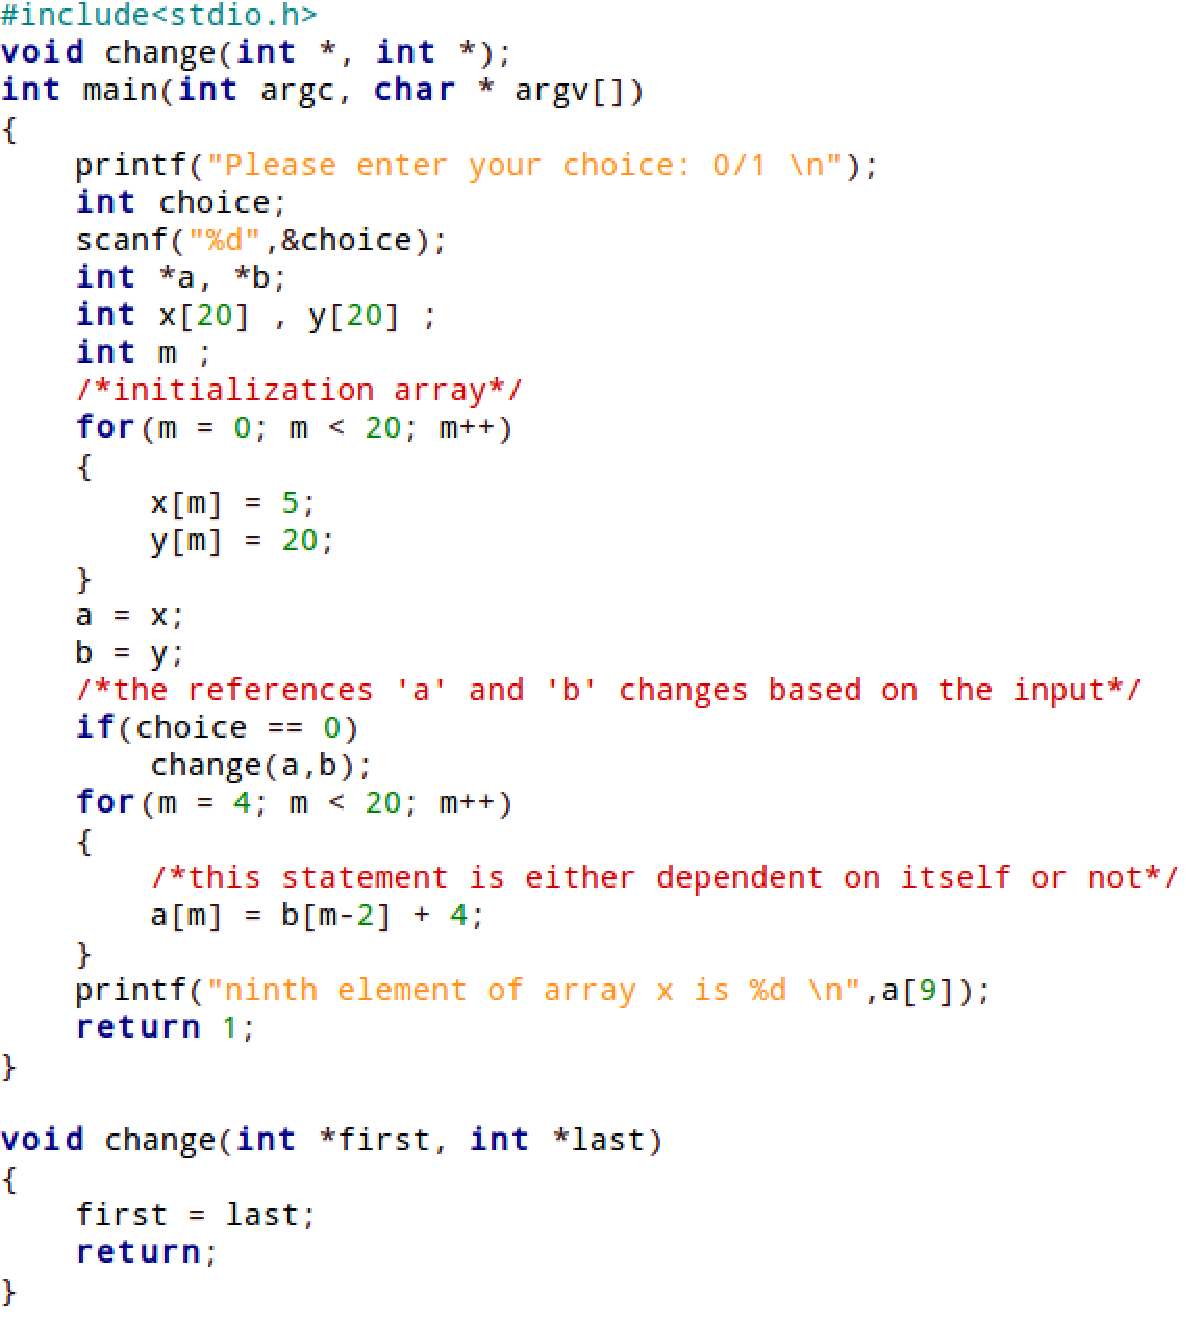
\includegraphics{./pdf/pointer.pdf}}
\caption{Code snippet for a loop where the alias relationship can't be determined at compile time.  The second \textit{for} loop in main can be either parallel or not based on the user input \textit{choice}.  Call to the function \textit{change} changes the alias relationship.}
\end{center}
\label{fig:example1}
\end{figure}

\begin{figure}[h]
\begin{center}
\scalebox{.5}{ 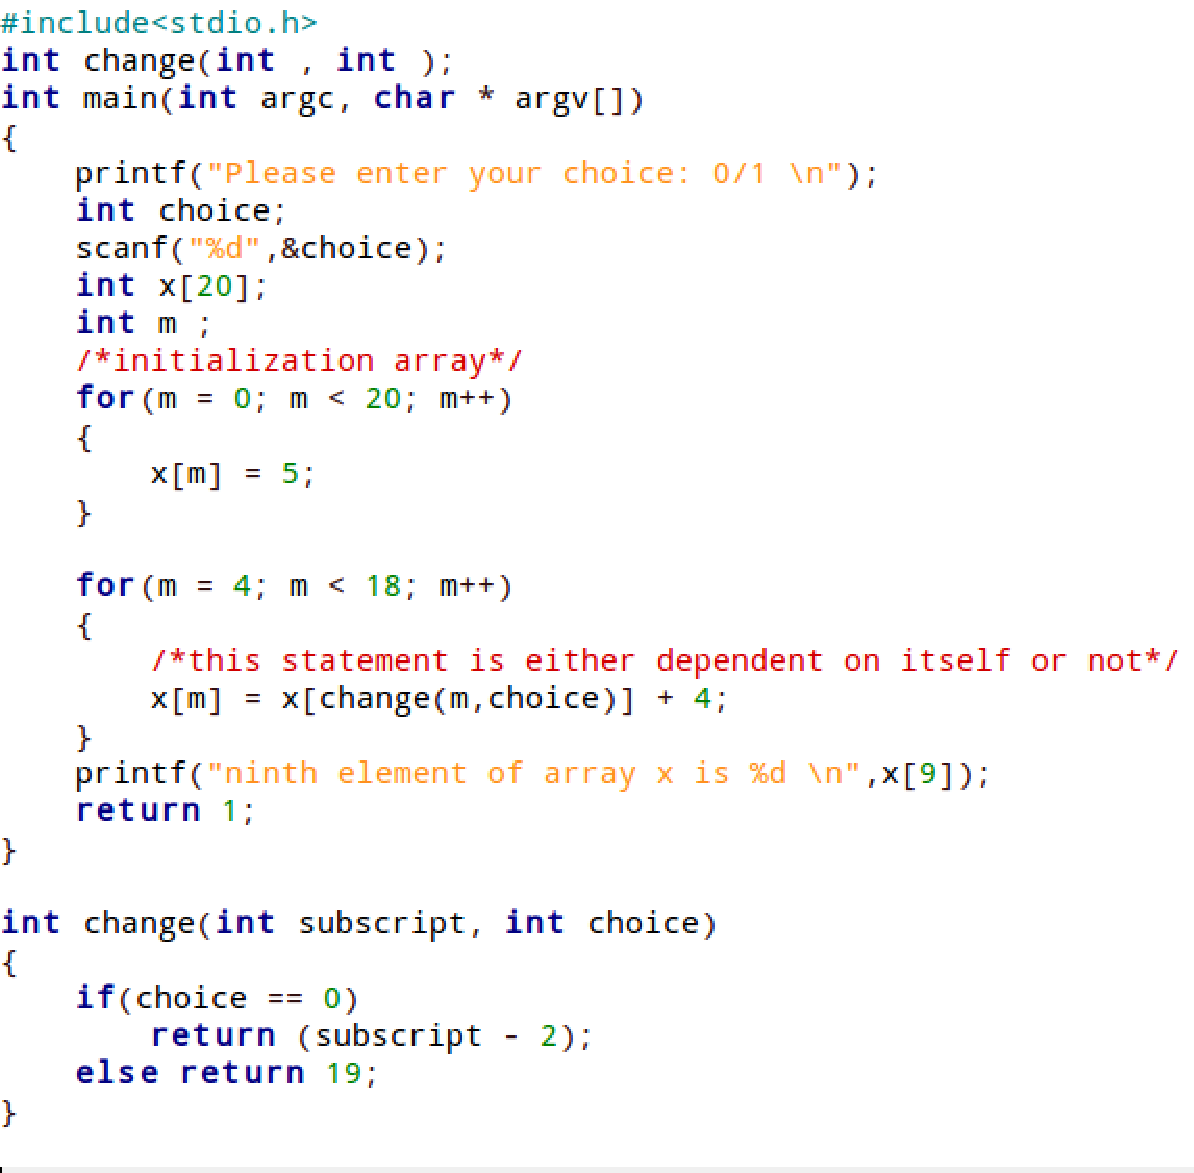
\includegraphics{./pdf/call.pdf}}
\caption{Code snippet for a loop where the alias relationship can't be determined at compile time.  The second \textit{for} loop in main can be either parallel or not based on the user input \textit{choice}.  Here the array subscript is a function call and the dependence analysis techniques reports this as a \textit{may} dependence.}
\end{center}
\label{fig:motv_exmp_2}
\end{figure}

Some dependence analysis use algebric techniques to find out the dependence behaviour of the loop. \cite{itest} \cite{lrpdtest} \cite{omega}  These techniques operate of array subscripts.  But they require the array subscripts to be \textit{affine} function of the loop induction variables.  If the subscript accesses another element or is determined by a function call, compilers can not prove the dependence at compile time and they report \textit{may} dependence. Figure \ref{fig:motv_exmp_2} demonstrates a program where the dependence relation of the statement inside the second \textit{for} loop of the \textit{main}  function is not provable at compile time because the subscript of the array is a function call that might change the alias relation(s). The function \textit{change} makes the loop either dependent or parallel based on user input.  Profiling of memory accesses come into play in these situations.

 
\section{Feedback directed Optimization}
\label{sec:fdo}

Feedback directed optimization (FDO) is a compiler optimization technique where the behaviour of the program is observed for some \textit{training} input.  The information gathered in the \textit{profiling} run is kept in a \textit{profile} file.  The profile file is read by the compiler in a subsequent analysis pass where different optimizations can be performed based on the profile information.  A typical feedback directed optimization is done in the following steps -

\begin{itemize}
\item \textbf{Instrumentation}\\
Compiler optimizations work on some Internal Representation (IR) of the source code.  The compiler front end converts the high level constructs of the source code to IR (language independent) for the middle end to work with it.  An instrumentation pass in FDO instruments the bitcode by adding calls to some profiling library functions so that the behaviour of interest can be captured.
\item \textbf{Profiling} \\
The instrumented bitcode is run with some training input and the output is stored in a profile file. 
\item \textbf{Optimization} \\
After the profiling run, an optimization pass is executed that takes both the original bitcode and the profile file as input and applies some code transformation based on the profiling data.  As a result of this pass, an optimized (may not be optimal) version of the bitcode is produced that in turn is translated to an executable by the back end.
\end{itemize} 

\subsection{Dependence Profiling}

Different behaviours of the program that can be captured with the help of profiling.  Some examples are \textit{edge profiling} (The execution frequency of the edges in the Control Flow Graph(CFG) of the program are profiled), \textit{path profiling} (the execution frequency of the different execution paths in the Call graph of the program are profiled), \textit{execution profile}  (Execution profile of the subroutines in the program that contains the execution time, resource consumption etc. by various routines in the program), \textit{power profiling} (power consumption by programs) etc. \\

\begin{figure}[h]
\begin{center}
\scalebox{.5}{ 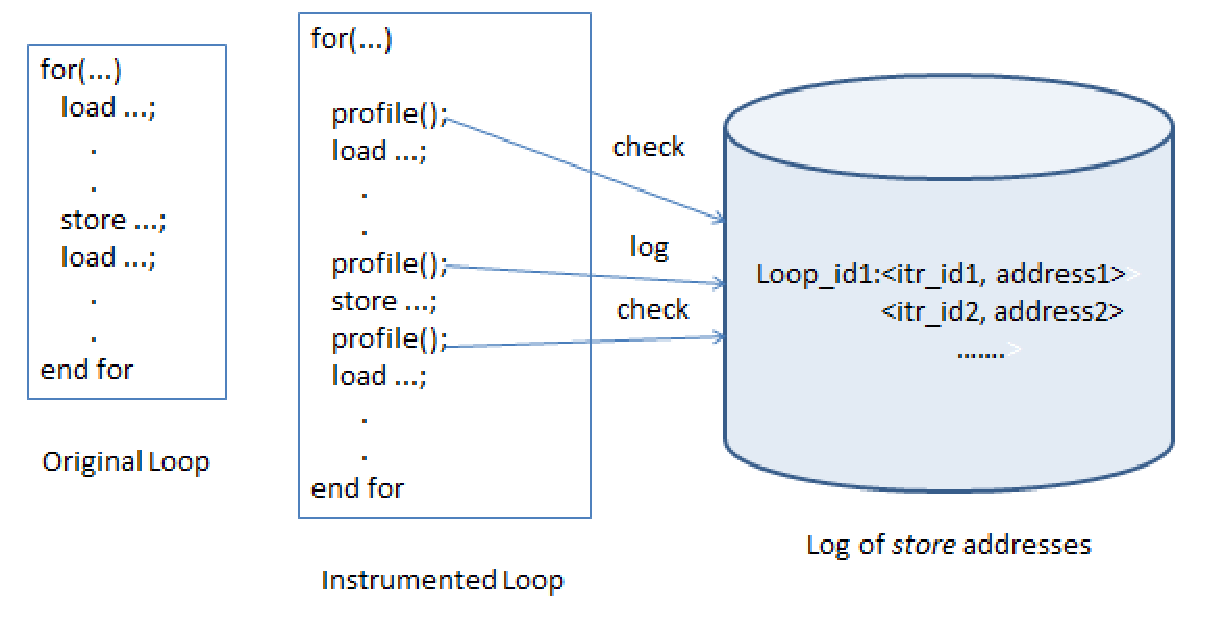
\includegraphics{./pdf/dep_profiler.pdf}}
\caption{An Example of a dependence profiler}
\end{center}
\label{fig:dep_profiler}
\end{figure}

Dependence profiling stores information about the different memory accesses by program parts.  For loops, the memory address accessed, the type of access (read/ write) and the iteration id for a particular loop is observed to find dependences.  The technique works by putting memory accesses by loads and stores in earlier iterations in a table (typically hash table for fast lookup).  Whenever a new load or store is executed, the table is searched to see whether the same address was accessed in a previous iteration.  If the same memory was accessed before, a new dependence is found. Figure \ref{fig:dep_profiler} demonstrates dependence profiling to find the RAW dependences in a loop.  Calls to the profiling library functions are inserted before every load and store instructions in the bitcode of the loop. For stores, the function logs a tuple <iteration id, memory address> in memory. Whenever a load is executed, the function checks in the log for a matching memory address to find a dependence.

\subsection{Cost of profiling}

Profiling comes with a cost.  There are two types of overhead:
\begin{enumerate}
\item Space Overhead
\item Time Overhead
\end{enumerate}
For dependence profiling, the memory overhead is huge if the memory accesses for the \textit{may dependent} statements across the \textit{whole} iteration space of the loop is stored.  Thus to reduce this overhead, the dependence analysis techniques normally work on \textit{loop samples} (some considerable portion of the iteration space) to get an approximation of the dependence behaviour.  Moreover, some compression techniques can also be applied to the storage required for profiling.\\
The timing overhead is optimized by either a fast lookup algorithm (e.g. hash table) and/or by creating smaller search space (with the use of access sets \cite{sd}).  For JIT(Just-in-time) compilers those use runtime profiling, time overhead is a major issue.  But for \textit{off-line} profiling (profiling done in a separate profiling run), the time is not a major issue, though profiling time should be reasonable.

\section{Combined Profiling}

Programs dependence behaviour changes according to the input to the program.  In the programs of figure \ref{fig:example1} and \ref{fig:motv_exmp_2}, for an input of '0', the second \textit{for} loop inside \textit{main}  \textit{cannot} be executed in parallel while for an input of '1', the loop can be parallel. But FDO has not achieved widespread use by compiler users because the selection of a data input to use for profiling that is representative of the execution of the program throughout its lifetime is difficult. For large and complex programs dealing with many use cases and used by a multitude of users, assembling an appropriately representative workload may be a difficult task. Picking one training run to represent such a space is far more challenging, or potentially impossible, in the presence of mutually-exclusive use cases. Moreover, user workloads are prone to change over time. Performance gains today may not be worth the risk of potentially significant performance degradation in the future.\\
Berube et al \cite{BerubeCP} proposed a method called Combined Profiling(CP) that eases the burden of training-workload selection while also mitigating the potential for performance degradation. First, there is no need to select a single input for training, because data from any number of training runs can be
merged into a combined profile. More importantly, CP preserves variations in execution behaviour between inputs. The distribution of behaviours can be queried and analyzed by the compiler when making code transformation decisions. \\
 The profile of a program records information about a set of program behaviours. A program behaviour
$B$ is a (potentially) dynamic feature of the execution of a program. The observation of a behaviour $B$ at a location $l$ of a representation of the program is denoted $B_l$ A behaviour
$B$ is quantified by some metric $M (B)$ as a tuple of numeric values. A monitor $R(B, l, M )$ is injected into a program at every location $l$ where the behaviour $B$ is to be measured
using metric $M$ . At the completion of a training run, each monitor records the tuple $<l, M (B_l )>$ in a raw profile.  In case of dependence profiling, the \textit{behaviour} to be observed is whether the loop is independent or not.  A \textit{monitor} is inserted inside every loop of the program and the \textit{metric} is the number of independent/ dependent executions.\\
CP stores the profile information with the help of histograms. Histograms are built in an incremental fashion in CP, thus removing the cost of storing multiple profile files that might increase the storage cost.  In general, updating produces a new histogram in 2 steps:

\begin{enumerate}
\item Determine the range of the combined data. Create a new histogram with this range.
\item Proportionally weight the bins of the new histogram.
\end{enumerate}

\begin{figure}[h]
\begin{center}
\scalebox{.5}{ 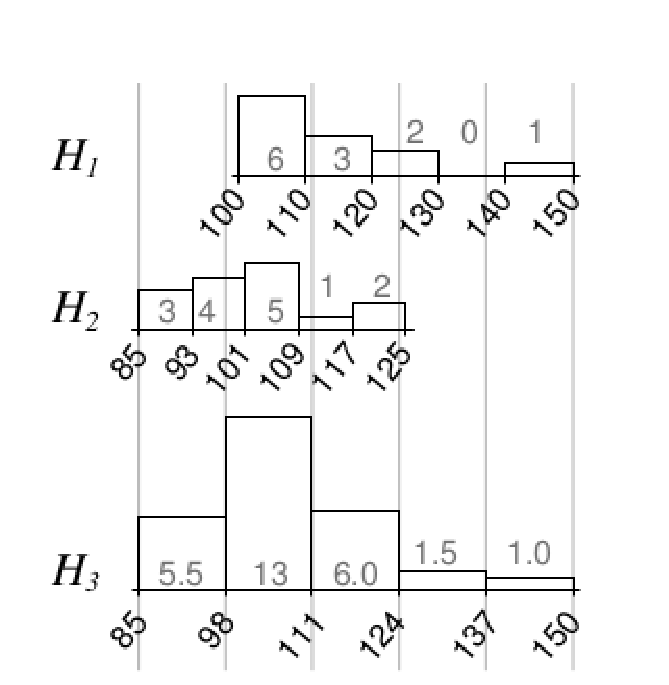
\includegraphics{./pdf/histogram.pdf}}
\caption{Combining histograms. $H_1$ has a bin width of 10
and a total weight of 12; $H_2$ has a bin width of 8 and a total
weight of 15. The combined histogram $H_3$ has a bin width
of 13 and a total weight of 27.
}
\end{center}
\label{fig:hist}
\end{figure}

The combination of two histograms $H_1$ and $H_2$ into a new histogram $H_3$ is illustrated in Figure \ref{fig:hist}. The range of $H_3$ is simply the minimum encompassing range of the ranges of $H_1$ and $H_2$ : $[min(100, 85), max(150, 125)] = [85, 150]$.
\\
This range is divided into the same number of bins as were present in the original histograms. The weight of a bin $b_i$ of $H3$ is given by the weights of the bins of $H_1$ and $H_2$ that overlap the range of bi multiplied by the overlapping proportion. For example, let $b_3$ be the third bin of H3 in
Figure \ref{fig:hist}. In $H_1$ the bin width is 10, and in $H_2$ the bin width
is 8. The weight of $b_3$ in $H_3$ is calculated as follows-

\begin{center}
$W_{b3}(H1) = (((120-111)\div 10)\times 3) + (((124-120)\div 10)\times 2)  = 3.5 $ \\
\end{center}
\begin{center}
$W_{b3}(H2) = (((117-111)\div 8)\times 1) + (((124-17)\div 8)\times 2)  = 2.5 $ \\
\end{center}
\begin{center}
$W_{b3}(H3) = (3.5 + 2.5) = 6.0$
\end{center}
  
\section{Thread Level Speculation}

This section describes the different concepts of TLS.
\label{sec:tls}

\subsection{Overview}
 
\begin{enumerate}
 
\item \textbf{Predecessor and Successor Threads} \\
Under the thread-level speculation (also called speculative parallelization) approach, sequential sections of code are speculatively executed in parallel hoping not to violate any sequential semantics.
The control flow of the sequential code imposes a total order on the threads. At any time during execution, the earliest thread in program order is non-speculative while the later ones can be speculative.
The terms \textit{predecessor} and \textit{successor} are used to relate threads in this total order.  In most schemes a squash rolls the execution back to the start of the thread, but some proposals in the literature use periodic checkpointing of threads such that upon a squash it is only necessary to roll the execution back to the closest safe checkpointed state. When the execution of a nonspeculative thread completes it commits and the values it generated can be moved to safe storage (usually main memory or some shared higher-level cache). At this point its immediate successor acquires non-speculative status and is allowed to commit. When a speculative thread completes it must wait for all predecessors to commit before it can commit.
\item \textbf{Inter Thread Data Dependence} \\
Data dependencies are typically captured by monitoring the data written and the data read by individual threads. A data dependence violation occurs when a thread writes to a location that has already been read by a successor thread. Dependence violations lead to squashing of thread, which involve discarding the side effects produced by the thread being squashed.
\item \textbf{Buffering of States} \\
Stores performed by a speculative thread generate speculative state that cannot be merged with the safe state of the program because this may lead to incorrect results. Such state is stored separately, typically in the cache of the processor. They are not written back to memory. In case of a violation is detected, the state is discarded from the cache. Also if a speculative thread overflows its speculative buffer the thread must stall and wait to become non-speculative. When the thread becomes non-speculative, the state is allowed to propagate (commit) to memory. When a non-speculative thread finishes execution, it commits. Committing informs the rest of the system that the state generated by the task is now part of the safe program state.
\item \textbf{Data Versioning} \\
A thread has at most a single version of any given variable. However, different speculative threads running concurrently in the machine may write to the same variable and, as a result, produce different versions of the variable. Such versions must be buffered separately. Moreover, readers must be provided the correct versions. Finally, as threads commit in order, data versions need to be merged with the safe memory state also in order to ensure correctness.
\item \textbf{Multi-Versioned Caches} \\
 A cache that can hold state from multiple tasks is called multi-versioned~\cite{Cintra00,Gopal,steffanISCA00}.\\
There are two performance reasons why multi-versioned caches are desirable: they avoid processor stalls when there is imbalance between tasks, and enable lazy commits.  
\end{enumerate}
 
 Speculative threads are usually extracted from either loop iterations or function continuations, without taking into consideration possible data dependence violations. The compiler marks these
structures with a fork-like spawn instruction, so that the execution
of such an instruction leads to a new speculative thread. The parent thread continues execution as normal, while the child thread is mapped to any available core. For loops, spawn points are placed
at the beginning of the loop body, so that each iteration of the loop spawns the next iteration as a speculative thread. Threads formed from iterations of the same loop (and that, thus, have the
same spawn point) are called \textit{sibling threads}. For function calls, spawn points are placed just before the function call such that the non-speculative thread proceeds to the body of the function, and a speculative thread is created from the function’s continuation~\cite{XekalakisICS09}. \\
Two different overheads should be considered when running loops speculatively in parallel.  The first overhead comes from buffering the state of the program before the start of speculative execution so that the program can be rolled back to a previous consistent thread.  If the computation done inside a thread is not large enough to overcome this cost, there is no benefit from speculation. \\
The overhead comes from the cost of misspeculation.  If there is actual dependence occurring between threads, the younger thread is squashed.  After a number of retries, the loop becomes sequential.  Thus if the probability is high that the loop is dependent, the loop should not be executed in parallel.
 
\subsection{TLS in IBM BlueGene/Q}

Bluegene/Q(BG/Q) is the latest IBM supercomputer in the Bluegene series (after BG/L and BG/P) that has hardware support for TLS and Transactional Memory(TM).  The initial objective of BG/Q was to include TLS support but later TM support was also added to it.  BG/Q requires hardware support for TLS, working in collaboration with a speculative runtime. The point of coherence for TLS in BG/Q is the L2 cache.  Each different version of a memory address can be stored in a different way of the L2 cache. When a write occurs for a speculative thread, the L2 allocates a new way in the corresponding set for the write. A value stored by a speculative write is private to the thread and is not made visible to other threads. The value is made visible to other threads when a thread commits and is discarded upon a thread squashing. In addition, the L2 directory records, for each memory access, whether it is read or written, and whether it is speculative. For speculative accesses, the hardware also tracks the thread that has read or written the line by recording the speculation ID used by the thread to activate speculation. This enables the hardware to detect conflicts among threads and also between speculative and non-speculative thread. \\
The IBM \textit{xlc} compiler has been modified to give speculation support in BG/Q and it is called \textit{bgxlc\_r}.  The \_r extension at the end generates thread safe code.  The following pragmas are used to speculatively execute a loop in parallel. \\
\textbf{\#pragma speculative for} \\
By default, if this pragma is used, iterations of the loop are divided into \textit{chunks} of size \textit{ceiling(number\_of\_iterations/number\_of\_threads)}. Each thread is assigned a separate chunk.\\
The following options can also be used with the \textit{\#pragma speculative for}:\\

$num\_threads (int\_exp)$ - The value of \ is an integer expression that specifies the number of threads to use for the parallel region.\\
$schedule (type)$- Specifies how iterations of the for loop are divided among available threads. Thread-level speculative execution supports static scheduling. Acceptable
values for type are as follows:\\
\textit{static} - Iterations of a loop are divided into chunks of size\\
\textit{ceiling(number\_of\_iterations/number\_of\_threads)}. This is the default scheduling policy. This scheduling policy is also known as block scheduling.\\
\textit{static,n}- Iterations of a loop are divided into chunks of size $n$. Each chunk is assigned to a thread in round-robin fashion. $n$ must be an integral assignment expression of value 1 or greater. This scheduling policy is also known as block cyclic scheduling. If $n=1$, iterations of a loop are divided into chunks of size 1 and each chunk is assigned to a thread in round-robin fashion. \\

\begin{figure}[h]
\begin{center}
\scalebox{.6}{ 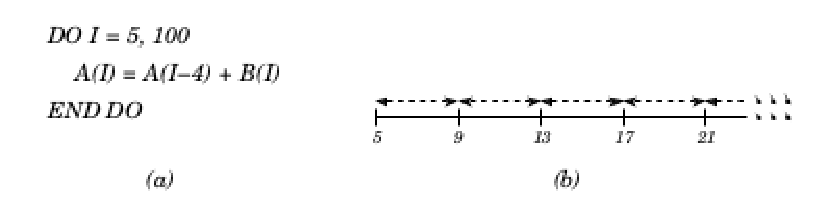
\includegraphics{./pdf/indep_window.pdf}}
\caption{An example where every 4 iterations of the loop can be executed in parallel}
\end{center}
\label{fig:indep_window}
\end{figure}

Figure \ref{fig:indep_window} shows an example where there is a \textit{strided} dependence pattern. (Dependence occurring at every fourth iteration of the loop).  Here every 4 iterations can be executed in parallel and into batches. The following pragma should be used in this scenario- \textit{\#pragma speculative for num\_threads(4) schedule(1)}.  While for using 2 threads pragma will be \textit{\#pragma speculative for num\_threads(2) schedule(2)}.  The $num\_threads$ and $schedule$ options should be carefully chosen to balance the overhead of thread creation.

\section{LLVM}
\label{sec:llvm}

The combined profiling and speculative parallelizing framework has been implemented in the LLVM compiler infrastructure.  LLVM has modular structure that makes the compiler easy to work with.  This section describes the different tools and passes those are useful for loop dependence analysis.

\begin{enumerate}

\item \textbf{The \textit{opt} tool}\\
The \textit{opt} tool of \textit{llvm} is useful to run different optimization-related passes.  There can be \textit{analysis} passes that performs analysis on IR constructs (like loops, CFGs, Call Graphs etc.) but does not modify the IR. The \textit{transformation} passes performs the actual transformations (e.g loop restructuring, Code motion etc.)
\item \textbf{Useful Passes}\\

\begin{itemize}
\item The \textbf{-scev} (ScalarEvolution) is an analysis pass that can be used to analyze and categorize scalar expressions in loops.  This pass specializes in recognizing general induction variables, representing them with the abstract and opaque
SCEV class.  Given this analysis, trip counts of loops and other important properties can be obtained. \\
\item The \textbf{-mem2reg} (Promote Memory to Register) is a transformation pass that converts non-SSA(static single assignment) form of LLVM IR into SSA form, raising loads and stores to stack-allocated values to "registers" (SSA values). Many of LLVM optimization passes operate on the code in SSA form and thus most probably will be no-op seeing IR in non-SSA form.\\
\item The \textbf{-loops} (Natural Loop Information) is an analysis pass that is used to identify natural loops and determine the loop depth of various nodes of the CFG.\\
\item The \textbf{-loop-simplify} is a transformation pass that performs several transformations on natural loops to change them into a simpler form, which makes subsequent analyses and transformations simpler and more effective. Loop pre-header insertion guarantees that there is a single, non-critical entry edge from outside of the loop to the loop header.  Loop exit-block insertion guarantees that all exit blocks from the loop (blocks those are outside of the loop that have predecessors inside of the loop) only have predecessors from inside of the loop (and are thus dominated by the loop header). \\
\item The \textbf{-memdep} pass is an analysis pass that performs memory dependence analysis.  This pass is based on the alias analysis pass.  The following types of alias analysis available in LLVM.
\item The \textbf{-basicaa} pass is an aggressive local analysis that knows many important facts like:
\begin{itemize}
\item Distinct globals, stack allocations, and heap allocations can never alias.
\item Globals, stack allocations, and heap allocations never alias the null pointer.
\item Different fields of a structure do not alias.
\item Indexes into arrays with statically differing subscripts cannot alias.
\item Many common standard C library functions never access memory or only read memory.
\item Function calls can not modify or references stack allocations if they never escape from the function that allocates them (a common case for automatic arrays).
\end{itemize}
\item The \textbf{-globalsmodref-aa} pass pass implements a simple context-sensitive mod/ref and alias analysis for internal global variables that don’t “have their address taken”. If a global does not have its address taken, the pass knows that no pointers alias the global. This pass also keeps track of functions that it knows never access memory or never read memory. The real power of this pass is that it provides context-sensitive mod/ref information for call instructions. This allows the optimizer to know that calls to a function do not clobber or read the value of the global, allowing loads and stores to be eliminated.
\item The \textbf{-steens-aa} pass implements a variation on the well-known "Steensgaard’s algorithm" for interprocedural alias analysis. Steensgaard’s algorithm is a unification-based, flow-insensitive, context-insensitive, and field-insensitive alias analysis that is also very scalable (effectively linear time). 
\item The \textbf{-scev-aa} pass implements AliasAnalysis queries by translating them into ScalarEvolution queries. This gives this pass a more complete understanding of pointer instructions and loop induction variables than other alias analyses have.
\end{itemize}
The dependence analysis reports \textit{may}, \textit{must} and \textit{no} dependence information.  Instrumentation is performed for the \textit{may} dependent instructions reported by the dependence analysis.  The next chapter describes the details of the combined profiling framework.
\end{enumerate}

\chapter{Combined Data Dependence Profiling}
\label{chapter:cp}

\section{Introduction}

Data dependence profiling is used to find out whether the \textit{may dependences} reported by the compiler by static analysis, materialize during run time.  This chapter describes how to use Combined Profiling~\cite{BerubeCP} in the case of data dependence profiling.  Combined data dependence profiles are built incrementally thus removing the necessity to store multiple profiles.  The combined profile file stores as much dependence information per loop as is necessary to perform a cost analysis to find speculation candidates.  A combined data dependence profiling framework implemented in the LLVM compiler infrastructure is described.  Results show that for benchmarks widely used in TLS literature, loops' dependence behaviour \textit{does not} change for different inputs.\\
Section \ref{framework} gives a high-level description of the framework.  Next in section \ref{LLVMImplementation} and \ref{library}, the different components of the framework are explained in details.

\section{The Framework}
\label{framework}

\begin{figure}[ht]
\begin{center}
\scalebox{0.6}{ \includegraphics{./pdf/framework_cp.pdf}}
\renewcommand{\figure}{Fig.}
\caption{ The Combined Data Dependence Framework implemented in LLVM}
\end{center}
\label{fig:framework}
\end{figure}

Figure \ref{fig:framework} shows the implemented framework.  First a \textit{transformation} pass \textit{profile-dependence} is run on the given source-code to instrument the later for profiling.  Also another \textit{analysis} pass \textit{printDbgInfo} is run to store the loop IDs and their corresponding file names and line numbers in a \textit{log} file.  Both of these passes need the bitcode to be produced with the debug information (-g option of clang).  Also the transformation pass needs three LLVM passes - \textit{mem2reg}, \textit{loops} and \textit{loop-simplify} (these passes are described already in~\ref{sec:llvm} of chapter 2). The instrumented bitcode is run with different inputs to produce a combined profile file \textit{llvmprof.out}.  This profile file can be consulted to find speculation candidate loops using different heuristics as described in later chapters.\\
The following sections give more details about the different components of the framework.


\section{The Instrumentation Pass}
\label{sec:instrumentation_pass}

The instrumentation pass performs IR instrumentation by adding calls to library-functions used for profiling.  This section describes the implementation details of the Instrumentation Pass.

\subsubsection{Choosing Loops}

The pass is written as a ModulePass in LLVM.  For a given bitcode, the pass iterates through all the modules.  For a given module, the pass iterates over the functions of the module and for a given function, the pass iterates over the basic blocks in the function. \\
In LLVM, the first basic block of a \textit{for} loop is named as \textit{for.cond$X$} where $X$ is any number (depends on the number of loops in the program).  Thus while iterating through the basic blocks of the function, if the pass finds a basic block with \textit{for.cond} in it's name, a variable \textit{loop\_count} is incremented. \\
The \textit{loop\_count} variable is used as a loop-identifier.  The variable is of type unsigned integer.  The variable is also used to create a unique global variable - \textit{iteration\_count} for each loop.  \textit{iteration\_count} is used in identifying the current iteration ID of the loop (as they will be needed later to calculate the dependence distance).  The iteration counter is cleared at the exit block of the loop so that the counter can be reused for another execution of the loop. \\
For being a speculation candidate, the loop has to have the following properties -

\begin{itemize}

\item Branching in or out of structured block and  parallel/work-sharing loop is not allowed. So if the loop has multiple exit blocks, the loop is not a speculation candidate.  Multiple exit blocks exist when there are one or more jumps (e.g. \textit{goto}-s) in the loop body.

\item The loop should be countable.  An example of non-countable loop is given in figure 1.2. 

\begin{figure}[h]
\label{fig:non_countable}
\begin{center}
\scalebox{.6}{ 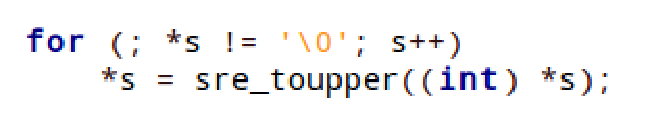
\includegraphics{./pdf/example_uncountable.pdf}}
\renewcommand{\figure}{Fig.}
\caption{ Example of a non-countable loop from \textit{hmmer} benchmark}
\end{center}
\end{figure}

\item If the loop has non-intrinsic function calls inside it's body, then the loop is not safe to parallelize.  But this constraint does not block a loop from executing speculatively in parallel.  The compiler can either relax the constraint or conservatively not parallelize loops with function calls.

\end{itemize}

\subsubsection{Implementation in LLVM}
\label{LLVMImplementation}
Different functions are used to check the above mentioned special characteristics of the loop.  This section gives the details of these functions.

\begin{itemize}

\item \textbf{Early exit condition of the Loop}\\
LLVM has a function, {\em getUniqueExitBlock}, that returns either the unique exit block of a loop or returns null if the loop has multiple exit blocks.

\item \textbf{Countable Loops}\\
The \textit{getSmallConstantTripCount}() function from the \textit{ScalarEvolution} pass is used to identify countable loops.  The function returns 0 if the trip count is unknown or not constant.

\item \textbf{Function Calls}\\
For checking if the loop body has function calls, the \textit{Call} instructions inside the loop body are identified.  If the call is to a C-library function, the body of the function will not be included in the bit code.  If the \textit{call} instruction is not a C-library call, the body will be there in the bitcode.  The \textit{empty}() function of LLVM's \textit{Function} class is used to make this distinction. If \textit{empty}() returns true, the \textit{call} is to a C-library function otherwise not.\\
After filtering out \textit{calls} to C-library functions, a check is necessary to check whether the function may access memory.  If the function may access memory, the loop is \textit{not} parallelized as the side effects of the function call may alter the dependence behaviour of the loop and an inter-procedural dependence analysis is necessary in that case.


\end{itemize}

\subsubsection{The Algorithm}

The instrumentation pass is implemented as A \textit{ModulePass} in LLVM.  Algorithm \ref{alg:InstrumentAlgo} is used for the instrumentation.  Basically the algorithm iterates over all the modules in the program and next all the functions in the module and lastly all the basic blocks in the function. \\
When the first basic block of the function is met, a void pointer is allocated that is used to store the different memory accesses by the \textit{load} and \textit{store} instructions those \textit{may} be dependent. This pointer is also used as an argument to the profiling functions.[Lines 4-6] \\
If the basic block's name contains "for.cond", the pass detects a loop.  Here we assume that no previous optimization(s) have been applied to the bitcode and all the loops' basic blocks are in the same order as the loops are met in the source code.  If a basic block is met with "for.cond" in its name, the $loopCount$ variable is incremented and two new global variables are also created. [Lines 8-13]

\begin{itemize}

\item \textbf{loop\_id} is an unique loop ID for the \textit{for} loop.
\item \textbf{iteration\_id} is required to identify the iteration number of the memory access.  This variable is incremented as we enter a loop body every time during the loop execution.  Also \textit{iteration\_id} is cleared at the exit from the loop so that the variable can be reused for the next execution of the loop \textit{for} loop.

\end{itemize}

Thus two global variables per loop are used. But only loops that have the properties as described in section \ref{LLVMImplementation} are instrumented.  The function \textit{candidateLoop}() checks for these properties.  The function takes the help of \textit{LoopInfo} and \textit{ScalarEvolution} passes of LLVM. \\
After creation of the global variables, the exit block of the loop is identified using the \textit{getUniqueExitBlock}() function.  As the loop is previously checked for having one exit block only, this function always returns a unique basic block.  Next, two instructions are inserted in the basic block.  The first one clears the \textit{iteration\_id} so that the variable can be reused in the next execution.  Another \textit{call} instruction  to the \textit{analyseAndWrite}() function is inserted. This function analyses the stored accesses to find the dependence pattern and write to profile  information. [Lines 14-17] \\
Next the loads and stores are identified and calls to the profiling functions are inserted accordingly.  There can be two types of basic blocks where the \textit{loads} and \textit{stores} can reside.  Either \textit{for.body} that comes just after the loop-conditional checking and \textit{for.end} that is the last basic block of the loop. \footnote{This condition happens when there is loop nesting and there are instructions in the outer loop after the execution of the inner loop}.  The loads and stores in these basic blocks are checked to see whether they are reported as \textit{may} dependent by the static analysis.  If they are, their memory accesses are stored in the \textit{void} pointer created before and a \textit{call} instruction to the profiling functions are inserted.  This function takes the memory address accessed, loop ID, iteration ID and the type of access (load/store) as parameters. More on this function is described later. [Lines 19 -29] \\
If the basic block is the loop body (\textit{for.body}), instructions to increment the \textit{iteration\_id} for the specific loop are also inserted. [Lines 30-33] \\
The collected profile is written to the profile file only once - during the exit from the program.  Now there can be two ways how a program can exit - 

\begin{itemize}

\item Return from \textit{main}
\item Calling the \textit{exit}() function from any functions.

\end{itemize}

So the instructions are checked in the basic block to see whether that is a \textit{return} instruction from \textit{main} or they are \textit{call} instructions to \textit{exit}() function.  If such instructions are met, a call to the function that accesses the profile file and write the collected profile information from memory to file is called. [Lines 35 - 49] \\
\begin{algorithm}
\begin{algorithmic}[1]
\FORALL {$mod$ in $Modules$}
	\FORALL {$func$ in $mod$}
		\FORALL {$basic\_block$ in $func$}
			\IF {$basic\_block$.$isFirstBasicBlockOfFunction()$}
				\STATE $allocateVoidPointer()$
			\ENDIF 
			\IF{$basic\_block.getName().contains(for.cond)$}
				\STATE loopCount++
				\STATE $loop$ = $getLoopFor$($basic\_block$)
				\IF {$loop$}
					\IF {$candidateLoop(loop)$}
						\STATE $createGlobal( loop\_id )$
						\STATE $createGlobal( iteration\_id )$
						\STATE $endBB$ = $getUniqueExitBlock(loop)$
						\STATE $createInstruction(makeIterationCountZero)$
						\STATE $createInstruction(callAnalyseAndWrite)$
						\STATE $insertInstructions()$
						\STATE
						\IF {$basic\_block.isLoopBody() || basic\_block.isLoopEnd()$}
							\FORALL {$instruction$ in $basic\_block$}
								\IF{$isMayLoad() || isMayStore()$}
									\STATE $createInstruction(getAddress(void_p))$
									\STATE $createInstruction(getLoopID())$
									\STATE $createInstruction(getIterationID())$
									\STATE $createInstruction(profileAccess())$
									\STATE $insertInstructions()$
								\ENDIF
							\ENDFOR
						\ENDIF
						\IF {$basic\_block.isLoopBody()$}
							\STATE {$createInstruction(incrementIterationCount)$}
							\STATE {$insertInstructions()$}
						\ENDIF
					\ENDIF
					
					\IF {$func == main$}
						\FORALL {$inst$ in $basic\_block$}
							\IF {$inst.isReturn() || inst.isCallToExit()$}
								\STATE $createInstruction(callWriteToFile())$
								\STATE $insertInstructions()$
							\ENDIF
						\ENDFOR	
					\ELSE				
						\FORALL {$inst$ in $basic\_block$}
							\IF {$inst.isCallToExit()$}
								\STATE $createInstruction(callWriteToFile())$
								\STATE $insertInstructions()$
							\ENDIF
						\ENDFOR
					\ENDIF

				\ENDIF
			\ENDIF
		\ENDFOR
		
	\ENDFOR
\ENDFOR
\caption{Instrumentation Algorithm}
\label{alg:InstrumentAlgo}
\end{algorithmic}
\end{algorithm}



\section{The Profiling Library}
\label{library}

In this section, the different functions and the data structures used in the profiling library are described.  

\subsubsection{Functions}

For each load and store instruction those are reported as may dependent by the static dependence analysis, a function call is inserted that behaves differently for loads and stores.  The following functions are the most important functions of the library. \\ 
\textit{void common(void * x,int count,int loop, char type)} is the main function that is used for dependence detection.  The working algorithm for this function is given in Algorithm \ref{alg:common_algo}. \\
The dependence behaviour is estimated from a portion of the loop's iteration space, the \textit{loop sample}.  The number of iterations to be considered for estimation is tunable by the macro \textit{MAX\_ITERATIONS}.  When this function is called for the first time, it performs a one time initialization of the data structures, this memory portion remains fixed for the whole profiling run.  This is static memory because dynamic memory location gives lots of memory fragmentation. \\
Until the \textit{loop sample} size is met, when a store in encountered, it is thrown in a bag, by the function \textit{add\_store}.  Since we only care about loads that depend on previous stores (RAW dependence), whenever a load is encountered, it is checked against the already captured store instructions for a given loop.  If the access addresses are same, a \textit{dependence pair} is found.  A dependence pair is defined as a tuple $(i_1,i_2)$ for a given loop where $i_1$ is the iteration ID of the store and $i_2$ is the iteration ID of the load. Note, $i_1$ is always less than $i_2$. Dependence pairs for that execution for that given loop are also kept.\\
When the loop enters an iteration ID that just exceeds the sample size; the collection of dependence pairs are analyzed to find the dependence behaviour.  If there are no dependence pairs, that means there were no RAW dependences for that execution of the loop and the loop's parallel execution count is incremented.  If there are some dependence pairs, the loop was not parallel for that execution.  As seen in figure \ref{fig:indep_window}, strided memory access patterns are interesting cases for parallel execution. The function $check\_stride()$ checks if there was a strided dependence pattern. The function uses the state machine described in figure \ref{fig:stride} to find strided dependence.  First the function calculates a dependence distance (distance between the iteration id of the write and that of read) for a given dependence pair. \\
Next the function checks for dependence pairs with the same dependence distance.  Every time such pair is encountered, a counter is increased.  If the counter value reaches a certain threshold (the threshold id set as 5) is reached, a strided dependence is reported, else the dependence becomes irregular. If there was a stride, the value of the stride is stored in the profile information, else the the loop has irregular dependence pattern. Also to reduce the search space, already visited dependence pairs are not searched again.\\

\begin{figure}[h]
\begin{center}
\scalebox{0.5}{ 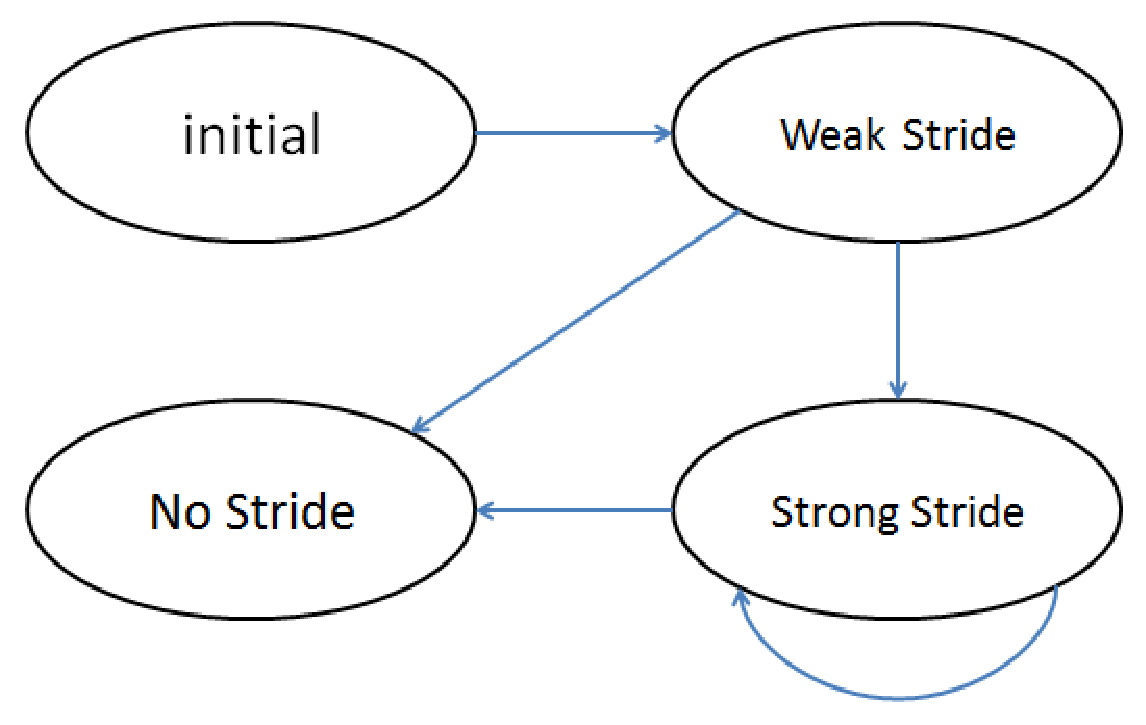
\includegraphics{./pdf/stride.pdf}}
\renewcommand{\figure}{Fig.}
\caption{ The State Machine for detecting strides}
\end{center}
\label{fig:stride}
\end{figure}


After analyzing and storing the dependence pattern in the memory for the given loop, all the data structures used in this execution of the loop is cleared so that they can be reused in the next run.  This is achieved by just clearing some counters, but not resetting the whole data structures.  Also the \textit{flag}, indicating that the dependence analysis is done, is set.\\
\textit{int analyse\_and\_write(int loop)} is used for the loops whose iteration count is smaller than \\ 
\textit{MAX\_ITERATIONS}.  This function is inserted at the exit block of the loop.  If the \textit{flag} indicating the dependence analysis is not set, then the function does the same operations as \textit{common()} does for iteration ids less than \textit{MAX\_ITERATIONS}.  Else the function just resets that flag for the next loop execution.  This function is useful for calculating dependence information for loops smaller than \textit{MAX\_ITERATIONS}.\\
\textit{int write\_to\_file()}  is called only when the program exists.  If there is already a profile file, this function updates the file using the information from the current run.  Else, the function creates a new profile file \textit{llvmprof.out}.  Call to this function is only inserted before the \textit{return} instruction from \textit{main} and before the \textit{call} instruction to the \textit{exit} function.  This function helps in reducing the cost of reading the profile each time a loop terminates.

\begin{algorithm}
\begin{algorithmic}[1]
\caption{Algorithm for the $common$ function, the common function finds dependence pairs and also characterizes the dependence as one of- \textit{strided}, \textit{irregular} or \textit{no-dependence}}
\label{alg:common_algo}
\IF{$iteration\_id <= MAX\_ITERATIONS$}
	\IF{data structures uninitialized}
		\STATE $initializeDS()$
		\STATE $setInitializedFlag()$
	\ENDIF	
	\IF {$load$ instruction}
		\STATE $check\_dependence()$
	\ELSE
		\STATE $add\_store()$
	\ENDIF
\ELSE
	\IF{$iteration\_id <= MAX\_ITERATIONS+1$}
		\IF {$dep\_pair\_count == 0$}
			\STATE loop parallel
		\ELSE
			\STATE $check\_stride()$
			\IF{stride found}
				\STATE strided dependence
			\ELSE
				\STATE irregular dependence
			\ENDIF
		\ENDIF
		\STATE $set\_analyzed\_flag()$
		\STATE $reset\_DS()$
	\ENDIF
\ENDIF

\end{algorithmic}
\end{algorithm}



\subsubsection{Data Structures}

This sections describes the various data structures those are used by the functions in the profiling library.\\
The data structure used by the library are \textit{static} arrays of structures.  Linked list is not a good choice here due to 1) The fragmentation created in the memory 2) They need an extra storage for storing the pointers to next and previous elements.  The different structures used are as follows. 


\begin{itemize}
\item \textbf{Memory Accesses} \\

struct Access \\
\{\\
	\hspace*{1 cm} int iteration\_id; \\
	\hspace*{1 cm} void * address;\\
\} \\
Only \textit{stores} need to be stored as the loads are checked on fly.  The $iteration\_id$ variable will always be less than $MAX\_ITERATIONS$.  A \textit{void} pointer is used to store memory address of any type.  A static array \textit{struct Access  stores [MAX\_LOOPS][MAX\_ACCESSES] }is used to store this information.  The $MAX\_LOOPS$ parameter is tunable and it gives the upper bound of the number of loops in a program. The value is set to 5000. $MAX\_ACCESSES$ gives the upper bound of the number of stores that can occur for an execution of the \textit{loop sample}.  The value is set to 2000.

\item \textbf{Dependence Pair} \\

struct DependencePair\\
\{\\
	\hspace*{1 cm} int write;\\
	\hspace*{1 cm} int read;\\
	\hspace*{1 cm} char checked;\\
\};\\

\textit{DependencePair} structure has three members.  $write$ and $read$ are used to store the iteration id of the store and load respectively.  $checked$ is a flag that is used during the stride calculation to avoid redundant computation.  A similar array \textit{struct DependencePair  pairs [MAX\_LOOPS][MAX\_DEPENDENCES]} is used to store the dependence pairs. 
\\
\textit{MAX\_DEPENDENCES} is also set to 2000.

\item \textbf{Profile Information} \\

struct Loop\_Info\\
\{\\
	\hspace*{1 cm} int loop\_id;\\
	\hspace*{1 cm} short parallel, irregular, first\_bin, second\_bin, third\_bin, fourth\_bin, fifth\_bin;\\
	
\};\\

$loop\_id$ stores the unique ID of the loop. $parallel$ and $irregular$ variables are used to store the number of parallel executions and the number of executions with irregular dependence.  The bins of the histogram are used to store the stride values for dependence.  An array \textit{struct Loop\_Info  info [MAX\_LOOPS]} is used to store the profile information in the memory.

\item \textbf{Miscellaneous Data Structures} \\

Apart from the main data structure mentioned above, the following arrays are also used -

\begin{enumerate}
\item To keep of the already analyzed \textit{flag}.
\item To keep track of the number of memory access count and dependence pair count.  These counters reduce the costly traversal of the arrays of data structures to prepare them for the next execution of the loop.
\item To store the discovered stride value, if applicable.
\end{enumerate}
\end{itemize}

The total size of the data structures remains fixed as they are initialized once and reused throughout the execution of the program.  For 5000 loops, 2000 accesses and 2000 dependence pairs, the memory overhead comes to 200 MB.

\section{The Profile file}

The profile file produced by the framework stores the dependence information for a number of executions for each loop. The combined profile file tries to capture as much dependence information as is necessary to perform a cost analysis to find speculation candidates.  There can be three types of dependences for a given loop.

\begin{itemize}
\item \textbf{No Dependence} If No dependence pairs are found for all the executions of the loop, the loop can safely be executed in parallel.
\item \textbf{Irregular Dependence} If the dependence does not follow any pattern (the dependence pairs have varied dependence distances), the loop is hard to parallelize.
\item \textbf{Strided Dependence} If the loop has a dependence with a stride value of 'n' (dependence is repeated for each 'n' iterations), every 'n' iterations of the loop can be executed in parallel, given the loop is doing significant work in those 'n' iterations to overcome the overhead from TLS.
\end{itemize} 

For each loop, the combined profile file stores the unique loop ID and the number of independent (parallel) and irregularly dependent executions.  The file also stores the different stride values in a histogram with five bins. 
Figure \ref{fig:profile_file} shows a sample profile file.\\

\begin{figure}[h]
\begin{center}
\scalebox{0.5}{ 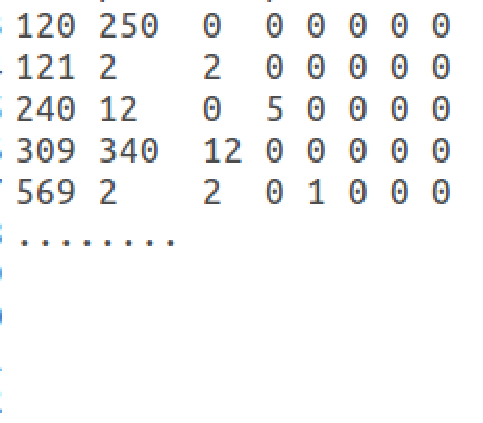
\includegraphics{./pdf/profile_file.pdf}}
\renewcommand{\figure}{Fig.}
\caption{ The structure of the profile file.  There are eight columns which represent loop\_id  parallel\_executions  irregular\_executions  first\_bin  second\_bin  third\_bin  fourth\_bin  fifth\_bin. The bins construct the histogram for storing stride values}
\end{center}
\label{fig:profile_file}
\end{figure}

\section{Variability of Loops' Dependence Behaviour based on Inputs}

One important finding of this research is that the dependence behaviour of loops that have the properties (as described is Section 4 of Chapter Background) to be speculation candidates, \textit{doesn't change} with respect to the different inputs to the program.  The dependence behaviour of loops from the SPEC2006, PolyBench/C and NAS benchmarks (as listed in  Table~\ref{table:benchmarks_observed}) is observed for different inputs and \textit{there was not a single loop that has the specific properties for being a TLS candidate and whose dependence behaviour varies with different inputs}. This finding allows the use of a simple heuristic for selection of speculation candidates based on profiling.  If the loop is dependent, the loop is not speculated.  If the loops is found to be independent, it is speculatively parallelized.  This invariability in the dependence behaviour also allows to use a single input for profiling and finding out TLS candidate loops.\\

\begin{table}
\centering
\caption{The Benchmarks observed to find loops with varied dependence behaviour }
\begin{tabular}{|c|c||c|c|} \hline
Benchmark Suite & Benchmark Name & Benchmark Suite & Benchmark Name \\ \hline 
Spec2006 & lbm & Spec2006 & h264ref \\ \hline
Spec2006 & hmmer & Spec2006 & mcf \\ \hline
Spec2006 & sjeng & Spec2006 & sphinx3  \\ \hline
Spec2006 & bzip2   & Spec2006 & gobmk  \\ \hline
Spec2006 & milc  & Spec2006 & namd   \\ \hline
PolyBench/C & 2mm	 &PolyBench/C & 3mm \\ \hline
PolyBench/C & gemm& PolyBench/C & gramschmidt\\ \hline
PolyBench/C & jacobi &PolyBench/C & lu	 \\ \hline
PolyBench/C & seidel &PolyBench/C & cholesky \\ \hline
PolyBench/C & dynprog &PolyBench/C & fdtd\_2d  \\ \hline
BioBench & mummer  &BioBench & protdist  \\ \hline
BioBench & protpar  &BioBench & dnapars  \\ \hline
BioBench & dnamove  &BioBench & dnapenny  \\ \hline
BioBench & dnacomp  &BioBench & dnainvar  \\ \hline
BioBench & dnaml  &BioBench & dnaml2  \\ \hline
BioBench & dnamlk  &BioBench & dnamlk2  \\ \hline
BioBench & dnadist  &BioBench & dollop  \\ \hline
BioBench & dolmove  &BioBench & dolpenny  \\ \hline
BioBench & restml  &BioBench & restml2  \\ \hline
BioBench & seqboot  &BioBench & fitch  \\ \hline
BioBench & kitsch  &BioBench & neighbor  \\ \hline
BioBench & gendist &BioBench & tigr  \\ \hline
BioBench & clustalw &BioBench & hmmer  \\ \hline
NAS & BT & NAS & CG  \\ \hline
NAS & DC & NAS & EP  \\ \hline
NAS & FT & NAS & IS  \\ \hline
NAS & LU & NAS & MG  \\ \hline
NAS & SP & NAS & UA  \\ \hline
\hline\end{tabular}
\label{table:benchmarks_observed}
\end{table}

\section{Benchmarks with loops that have varied dependence behaviour across inputs}

In this section description of three different benchmarks, that have loops with varied dependence behaviour across different executions, are given.
\begin{itemize}
\item \textbf{2D-Hull:} The randomized incremental algorithm that builds the Convex Hull of a two-dimensional set of points is used. This algorithm, called 2D-Hull (due to Clarkson et al. [23]), computes the convex hull (smallest enclosing polygon) of a set of
points in the plane. The input to Clarkson's algorithm is a set of (x, y) point coordinates. The algorithm starts with the triangle composed by the first three points and adds points in an incremental way. If the point lies inside the current solution, it will be discarded. Otherwise, the new convex hull is computed. Note that any change to the
solution found so far generates a dependence violation, because other successor threads may have been used the old enclosing polygon to process the points assigned to
them.\\
The probability of a dependence violation in the 2D-Hull algorithm depends on the shape of the input set. For example, if N points are distributed uniformly on a disk, the i-th iteration will present a dependence with probability in θ(√i/i). If points lie uniformly on a square, the probability of a dependence will be in θ(log(i)/i).

\item \textbf{Delaunay triangulation:} The second application is the randomized incremental construction of the Delaunay triangulation using the Jump-and-Walk strategy, introduced by Mucke et al. [24], [25]. This incremental strategy starts with a number of points, called anchors, whose containing triangles are known. \\
The algorithm finds the closest anchor to the point to be inserted (the jump phase), and then traverses the current triangulation until the triangle that contains the point to
be inserted is found (the walk phase). After this location step, the algorithm divides this triangle into three new triangles, and then updates the surrounding edges to
keep the Delaunay properties.\\
This local modification to the current Delaunay solution may lead to dependence
violations, since other threads may have traversed the old solution while trying to add new points. The shared data access pattern of the Delaunay algorithm is fundamentally different than the one of the 2D-Hull. In the Delaunay algorithm all threads modify the
speculative solution, not only a subset of them. However, despite these modifications, successor threads do not need to be squashed if their own work is carried out
in a different zone of the triangulation.\\
The expected amount of dependence violations generated by the Delaunay Triangulation depends on the number of processors and the length of the traversing path. It is easy to see that, the shorter the distance between the closest anchor and the point to be inserted, the fewer triangles that are visited in the walk and the smaller the probability of a dependence violation. This fact suggests that the algorithm should work with many anchors. However, the bigger the number of anchors, the more distance comparisons have to be performed to find the closest anchor to our point, thus degrading sequential performance. Our implementation uses a number of anchors that represents a good balance between these effects for the input size used. Our implementation is
composed by two loops: The first one builds a Delaunay Triangulation of the first 5 000 points, that will be used later as anchors, while the second loop inserts all the
remaining points (up to one million). We have speculatively parallelized this second loop.
\end{itemize}

\chapter{A framework for automatic speculative parallelization of loops using polyhedral dependence analysis}
\label{chapter:polly}

\section{Introduction}

The fact that loops' dependence behaviour does not change based on inputs for the benchmarks used in TLS literature, makes it easier to choose candidate loops for speculative execution. This chapter presents an automatic speculative parallelization framework built on \textit{Polly}~\cite{grosserImpact11}, the polyhedral optimizer in LLVM.  The framework uses Polly's dependence analyzer to find may dependences in the loops.  Two different heuristics are used to find speculation candidates. The first heuristic allows loops with only may dependences to run speculatively in parallel while the second heuristic filters out cold loops and, using profile information, loops with actual run time dependences. A performance evaluation of the speculative code generated by the framework over the sequential version at the lowest optimization level (-O0) for the SPEC2006 and PolyBench/C benchmarks is presented.

\section{Speculative Parallelization using the polyhedral dependence analyzer of LLVM}
\label{section:heuristics}

This section describes the two heuristics used by the framework to find speculation candidate loops.  

\subsection{Heuristic 1}

According to the first heuristic,  for being a speculation candidate a \textit{SCoP} (loop) should have only \textit{may dependences}. The goal of this heuristic is to relax the constraint for OpenMP parallelization (OpenMP does not parallelize loops with \textit{may dependences}) and find more parallelization candidates.  The hope is that the \textit{may dependences} will not materialize at run time, thus resulting in speedup. 
 
\subsection{Heuristic 2}

Heuristic 1 allows loops with \textit{may dependences} to execute in parallel.  There can be two cases where the overhead of speculation can still negate the gain from parallelism. In heuristic 2, the two criteria for filtering are based on two different overheads. The first criteria considers the overhead from mispeculation and recovery while the second criteria considers the overhead from thread creation and storing the program state so that the system can be rolled back to a consistent state in case of mispeculation.  In this way loops that can not be benefited from SE are filtered. 

\begin{enumerate}
\item In the loops where \textit{Polly} reports only \textit{may dependences}, the memory accesses are profiled for a training run for some inputs.  If the training run shows that the \textit{may dependences} are materializing into \textit{actual dependences} at run time, the loop is not parallelized.
\item If the execution time of the loop is less than some threshold as compared to the total execution time of the program, the loop also is not speculatively parallelized.  As in this case, the overhead from speculation can neutralize or, worse, negate the gain from parallelism. This threshold is set as 20\% of the total execution time because experimental evaluation shows that allowing  the speculative execution of smaller loops for the benchmarks leads to slowdown. 
\end{enumerate}

\section{The Framework for Polly}
\label{section:framework}

The framework is implemented in the LLVM~\cite{llvm} compiler infrastructure. Polyhedral dependence analysis is already implemented as a part of the LLVM project and it is called \textit{Polly}~\cite{grosserImpact11}. \\

\begin{figure}[h]
\begin{center}
\scalebox{0.35}{ 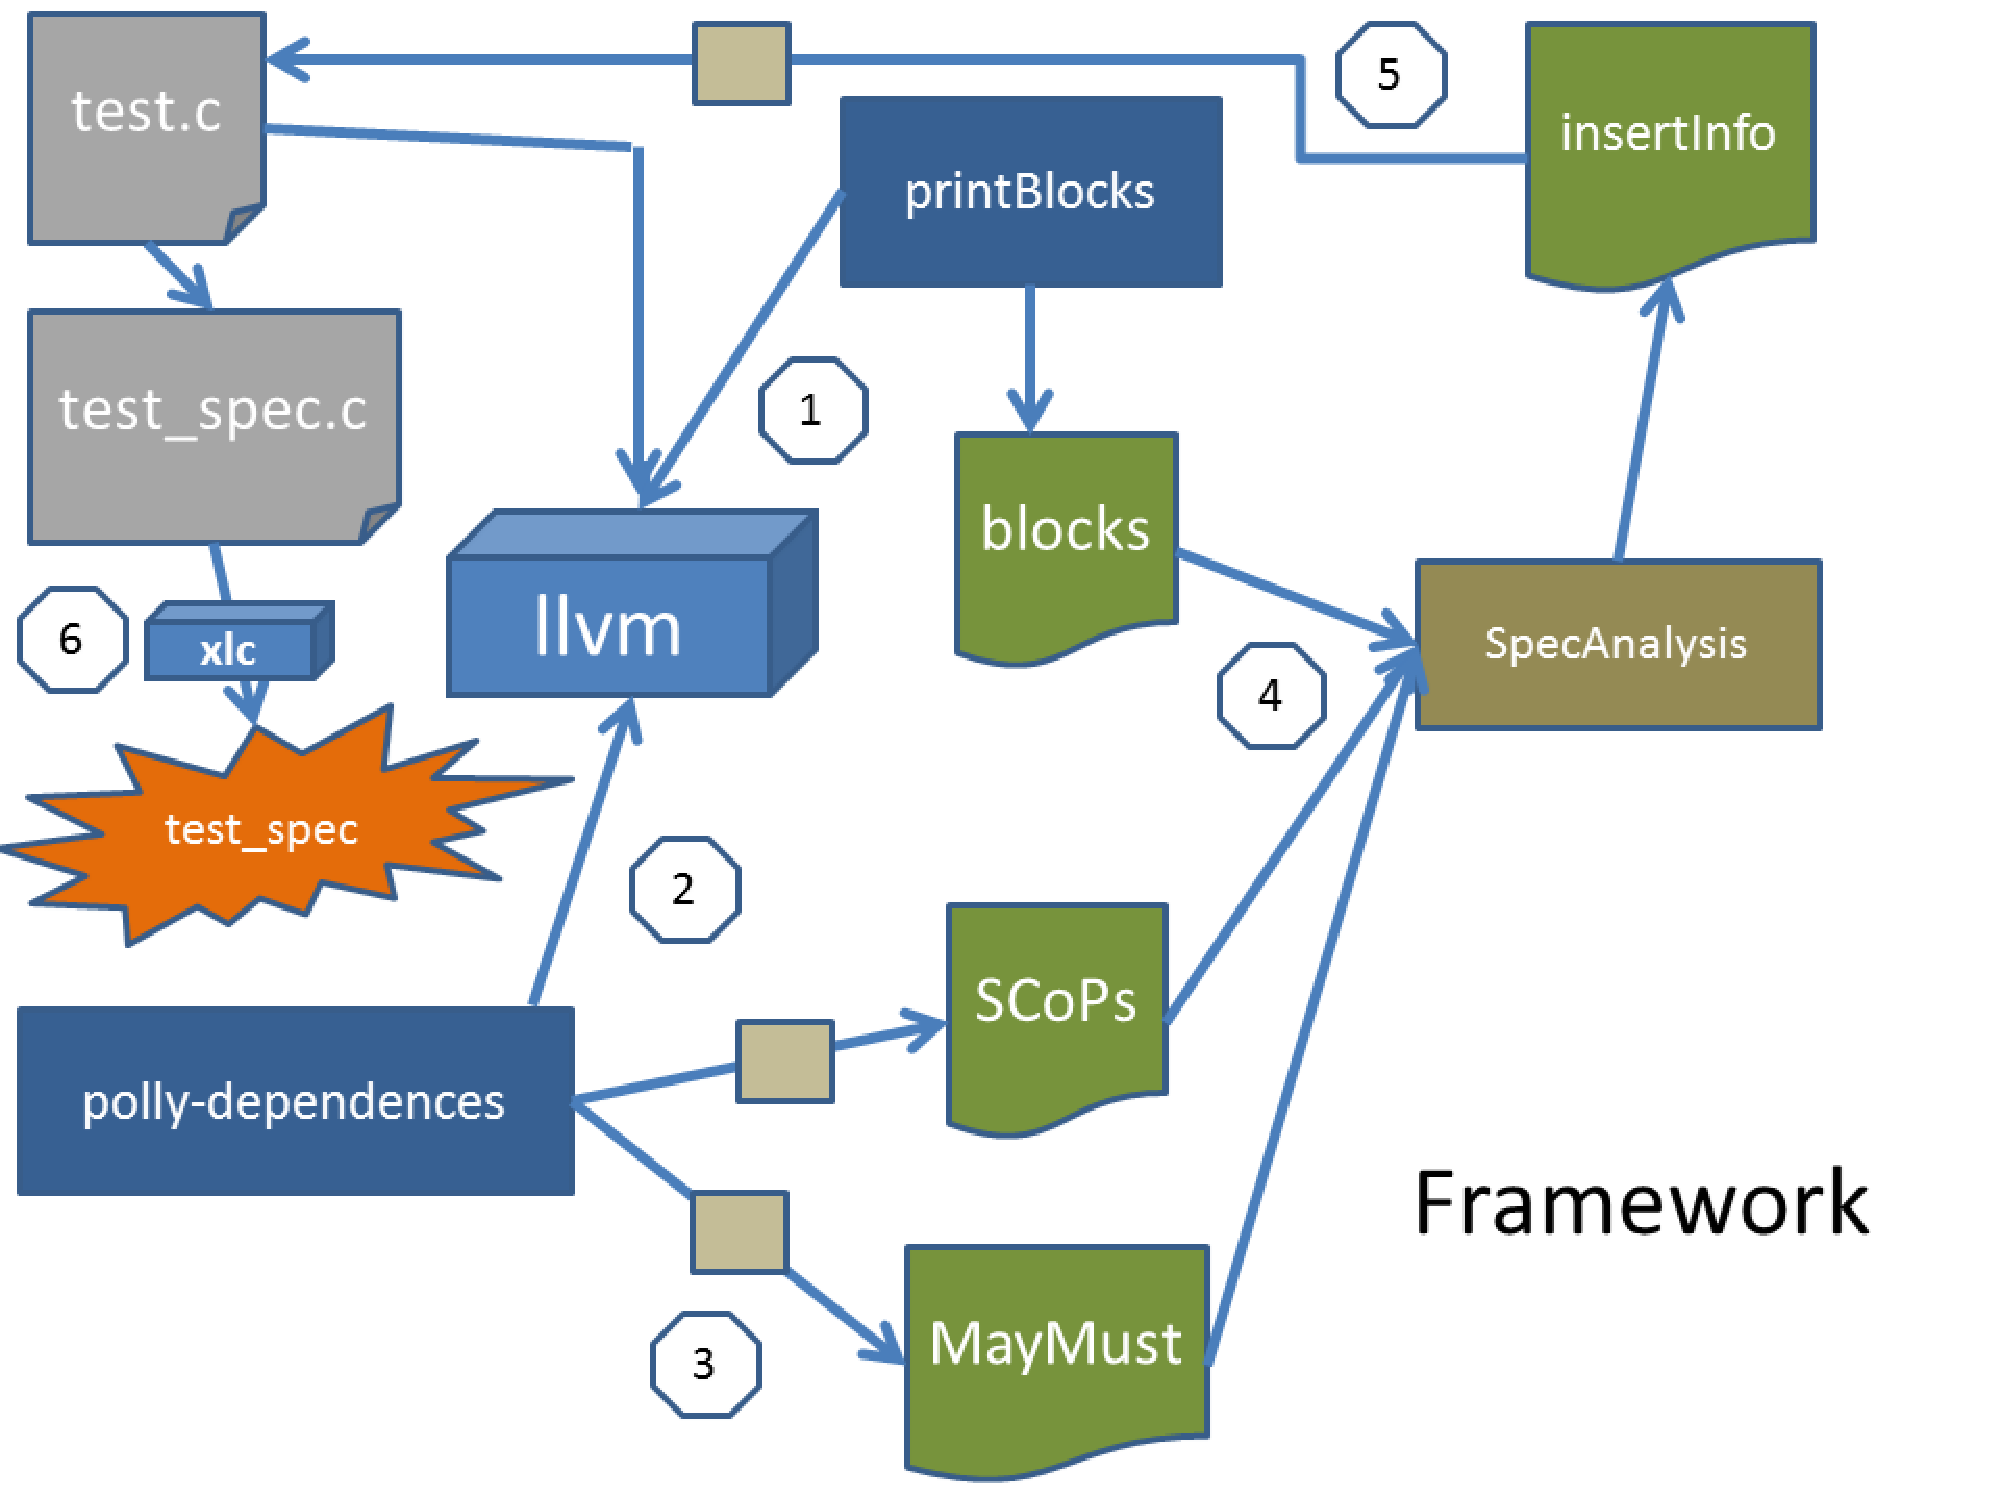
\includegraphics{./pdf/framework.pdf}}
\renewcommand{\figure}{Fig.}
\caption{ The Framework}
\end{center}
\label{fig:framework_polly}
\end{figure}

First the source-code file to be optimized is compiled with LLVM keeping the debug information in the bitcode (with -g option). The debug information is necessary for source-code instrumentation.  Two LLVM passes are run on the generated bitcode. The \textit{printBlocks} pass prints out all the basic blocks in the source file and their corresponding file name and line numbers.\\

Polly's dependence analysis pass \textit{Polly}-\textit{dependences} is also run on the bitcode.  This pass provides information about the SCoPs and the \textit{may} and \textit{must dependences} in them.  This dependence information is extracted from the output and kept into temporary storage.  An analyzer program takes the information generated by the above two passes as input, performs a three-way mapping (SCoPs with basic block information, basic block with file name and line numbers information and SCoPs and dependence information), performs analysis based on which heuristic to use and outputs information about the file names and line numbers where the speculative \textit{pragmas} can be inserted. A script is run that reads the file name and line numbers and instruments the code accordingly.  For the benchmarks tested, the number of loops never exceeds 6000 (the maximum number of candidate loops for speculation are much less than that) and the temporary storage necessary was less than 5 MB.  Figure~\ref{fig:framework_polly} describes the framework.\\

The instrumented source code is then compiled with the \textit{bgxlc\_r} (\_r option generates thread-safe code. \textit{bgxlc} is the IBM xlc compiler specific for the BlueGene/Q machine) compiler to generate the executable that can be run on the BlueGene/Q ~\cite{BGQ} machine.  The framework is fully automatic.

\section{Experimentation}

Experimentation is performed on two different sets of benchmarks - SPEC2006 benchmarks~\cite{spec}  and the PolyBench/C benchmarks~\cite{polybench}.  SPEC2006 is chosen because it has been used by other researchers for the evaluation of speculative execution. All the SPEC2006 benchmarks are not reported because some of them don't run successfully on BlueGene/Q.  PolyBench/C benchmarks are chosen because they are suitable benchmarks for polyhedral analysis.  Table \ref{table:bgq_config} shows the hardware details of a BlueGene/Q chip. \\
 
The SPEC2006 benchmarks are run with the \textit{ref, train and test} input and the PolyBench/C benchmarks are run using varied problem size.  For calculating the speedups, each benchmark is run 15 times for a given input and the average running time from the 15 runs were taken. For runs with profiling, there are three groups of 5 runs and for each group, the input for the profiling run is different from the input for the measurement run. Also the 95\% confidence interval is shown in the bar chart for the 15 runs.\\

Instrumentation in the source code is done automatically following the information file generated by the framework.  The \textit{\#pragma speculative for} pragma from the IBM \textit{bgxlc\_r} compiler was used for speculative execution of loops.  This pragma divides the iterations of a loop into chunks of size
$ceiling(number\_of\_iterations/number\_of\_threads)$. \\

The loop must be countable at compile time to be a speculation candidate.  Each thread is assigned a separate chunk.\\

The baseline for comparison is the sequential version of the benchmarks compiled with the -O0 optimization level of the \textit{bgxlc\_r} compiler.  The lowest optimization level ensures that the optimization of hot loops (-qhot) and automatic SIMDization of the sequential code (-qsimd=auto) is turned off. For comparison with the OpenMP version, the automatic OpenMP code generated by \textit{Polly} for the benchmarks is used.  Polly inserts calls to OpenMP runtime functions to automatically parallelize independent SCoPs. Still the automatic OpenMP version generated by Polly can be worse than the OpenMP version of the code written by the programmer.


\begin{table*}
\centering
\caption{Configuration of a BluGene/Q chip}
\begin{tabular}{|c||c|} \hline
\#Processors&17(16 User and 1 service PowerPC)\\ \hline 
Multithreading&4-way Multithreaded \\ \hline
Clock&1.6GHz \\ \hline
L1 I/D Cache&16KB/16KB \\ \hline
Peak Performance & 204.8 GFLOPS \@ 55W \\ \hline
RAM&16 GB DDR3 \\ \hline
Multiversioned Cache & Support for Transactional Memory and Speculative Execution \\ \hline
L2 Cache & Centrally shared, 32 MB \\ \hline
Chip-to-chip networking & 5D Torus topology + external link \\ \hline
\hline\end{tabular}
\label{table:bgq_config}
\end{table*}

\section{Results}
\label{section:results}

This section describes the experimental results for the experimentation with \textit{Polly}.  First the effect of heuristic 1 on the SPEC2006 and the PolyBench/C benchmarks is described.  Then a comparison between OpenMP parallelization and the parallelization done by the framework following heuristic 1 is presented.  The effect of heuristic 2 on the two sets of benchmarks is also shown.  Results show that data dependence profiling is necessary because in benchmarks like \textit{sjeng}, may dependences materialize during runtime and cause a slowdown. The results also show that speculatively parallelizing loops that have poor coverage (percentage of the whole program execution time) results in slowdown for benchmarks like \textit{fdtd-2d}, \textit{jacobi}, \textit{lu}, \textit{seidel}, \textit{cholesky}, \textit{dynprog}, \textit{gramschmidt}, \textit{gobmk}.  Applying heuristic 2 to filter out loops with actual dependences and cold loops (less than 20\% coverage) gives performance improvement over automatic OpenMP parallelizer of \textit{polly} for \textit{gramschmidt} and \textit{sjeng}.

\subsection{Heuristic 1}

\subsubsection{Spec2006 Benchmarks}

\begin{figure*}
\begin{center}
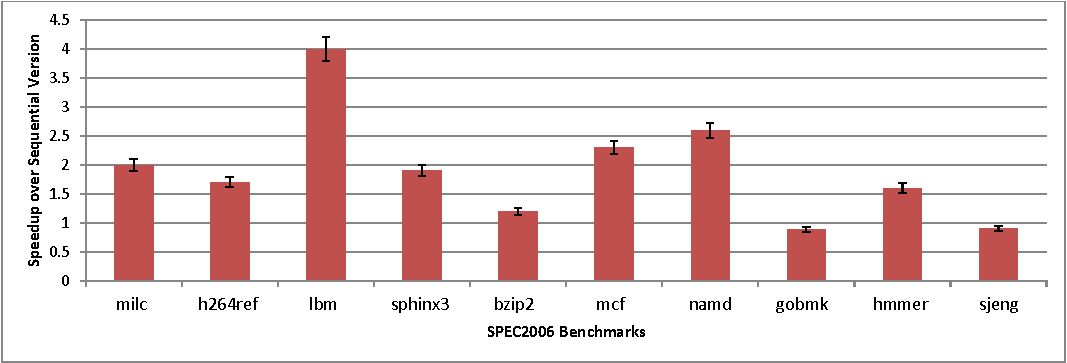
\includegraphics[scale =0.75]{./pdf/speedup_spec2006.pdf}
\caption{Speed up of the instrumented SPEC2006 benchmarks over the optimized sequential version on a 8 node cluster. Most of them gets a speedup, the maximum being \textit{lbm} due to the presence of a large parallelizable loop. \textit{gobmk} suffers a slow down because of the presence of many loops with small iteration count. \textit{sjeng} also offers a slow down because the \textit{may} dependences actually occur during run time. Dependence profiling can be done to eliminate those candidate loops with \textit{may dependences} for \textit{sjeng}.}
\end{center}
\label{fig:speedup_spec2006}
\end{figure*}

In Figure~\ref{fig:speedup_spec2006}, most of the SPEC2006 benchmarks achieve a speedup over the optimized sequential version.  \textit{lbm} contains loops with no inter-thread data dependences, but these dependences are not statically provable by the compiler and that's why they are not parallelized by OpenMP. This benchmark can be greatly benefited by the speculative execution and obtains the highest speedup because these dependence don't materialize at run time.\\
\textit{gobmk} has many loops with small iteration counts. Small loops are not good candidates for speculative execution because the thread creation overhead negates the impact of parallel execution and we get a slowdown. These loops are later filtered out by heuristic 2.\\
\textit{sjeng} contains loops those are reported as speculation candidates by heuristic 1 because of the occurrence of \textit{may dependences}.  But these dependences actually occur at run time and the overhead from mispeculation prevents this benchmark from achieving speedup.  These loops are not suited for speculative execution and they are eliminated by heuristic 2.\\
Overall, heuristic 1 performs well for most of the SPEC2006 benchmarks.  A 4x speedup is achieved for \textit{lbm} benchmark on a 8-node cluster. 

\begin{figure}[h]
\begin{center}
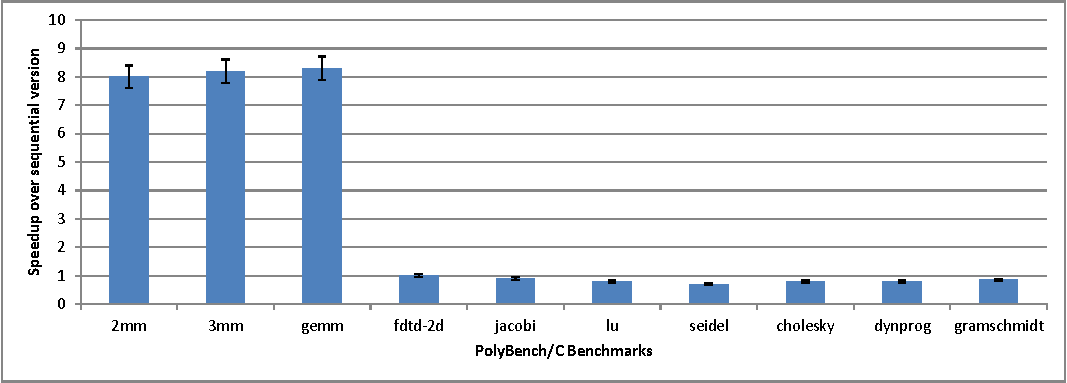
\includegraphics[scale =0.75]{./pdf/speedup_polybench.pdf}
\caption{Speed up of the instrumented PolyBench/C benchmarks over the optimized sequential version on a 12 node cluster. The last five benchmarks suffers a slow down because of launcing threads for loops with small iteration count and also parallelizing loops in the innermost level (finer granularity)}
\end{center}
\label{fig:speedup_polybench}
\end{figure}

\subsubsection{PolyBench/C Benchmarks}

The speedups reported in Figure~\ref{fig:speedup_polybench} indicate that the  PolyBench/C programs can be divided into two classes according to the effectiveness of thread-level speculation. Class 1 contains programs\textit{ 2mm, 3mm, correlation, covariance, doitgen, gemm} that achieves speed up on a speculative execution and Class 2, containing \textit{gramschmidt, jacobi-2d-imper, lu, ludcmp, seidel} experiences a slow down.  In the Class 2 PolyBench/C programs the loops parallelized are very small and constitutes a very small portion of the overall program execution (mainly initialization arrays).\footnote{These results confirm the finding of Kim et al.~\cite{sd3}}  Therefore the overhead for thread creation in the speculative execution negates the performance achieved from the parallel execution of these loops. Table \ref{table:coverage_1} shows the percentage of the whole program execution time the parallelized loops take for the PolyBench/C benchmarks. For \textit{seidel} the coverage is only 0.04\% and therefore the loops are not good speculation candidates for this benchmark.  The cold loops are eliminated by heuristic 2.

\subsection{Comparison with OpenMP Parallelization}

Heuristic 1 relaxes the constraint of OpenMP parallelization and allows loops with \textit{may dependences} and no \textit{must dependences} to speculatively run in parallel too.  As seen in Table ~\ref{table:coverage_1}, heuristic 1 is able to find more parallelization candidates than OpenMP parallelization for the PolyBench/C benchmarks.  Figure~\ref{fig:openmp_vs_spec_poly} shows the speedup gained from OpenMP parallelization and speculative parallelization for the PolyBench/C benchmarks.  For \textit{2mm} and \textit{3mm}, speculative optimization does not give better speedup because no new loops are discovered by the framework.  For the last five benchmarks, OpenMP performs better than speculative optimization because the loops parallelized by heuristic 1 in the benchmarks are pretty small and they take very small portion of the benchmark execution time.  Therefore executing them speculatively causes the overhead from TLS to negate the gain from parallel execution.  The slowdown in these benchmarks are the motivation for heuristic 2.\\
Most of the time the framework outperforms OpenMP for the SPEC2006 benchmarks, as can be seen in Figure~\ref{fig:openmp_vs_spec}.

\begin{table}
\centering
\caption{Number of Loops parallelized by OpenMP parallelism vs Speculative parallelism using heuristic 1.  As heuristic 1 allows loops with \textit{may dependences} and no \textit{must dependences} to be executed in parallel as well, the heuristic was able to find more parallelizable loops.}
\begin{tabular}{|c||c|c|c|c|} \hline
Benchmark &Total & OpenMP & Speculative & Coverage\\ \hline 
lbm & 23 & 1	 & 4 & 97 \\ \hline
h264ref & 1870 & 250	 & 120 & 79  \\ \hline
hmmer &	851	 & 30 & 45 & 72 \\ \hline
mcf & 52 & 2 & 4 & 60 \\ \hline
sjeng &	254 & 16	 & 3 & 12 \\ \hline
sphinx3 & 609 & 11 & 2 & 91 \\ \hline
bzip2 & 232 & 4 & 2 & 35 \\ \hline
gobmk & 1265 & 0 & 1 & 13 \\ \hline
milc & 421 & 5 & 20 & 68 \\ \hline
namd & 619 & 7& 20 &92 \\ \hline
2mm	&20& 7 &7 & 99 \\ \hline
3mm	&27& 10&10 & 99 \\ \hline
gemm	 &13& 3&4 & 98 \\ \hline
gramschmidt	&10& 2&3 & 1 \\ \hline
jacobi & 9&	3& 3 & 2 \\ \hline
lu	& 8 & 1 & 2 & 2 \\ \hline
seidel&	7& 1 & 1 & 0.04 \\ \hline
cholesky & 9 & 0 & 1 & 2  \\ \hline
dynprog & 9 & 7 & 2 & 13 \\ \hline
fdtd\_2d & 14 & 2 & 0 & - \\ \hline
\hline\end{tabular}
\label{table:coverage_1}
\end{table}

\begin{figure*}
\centering
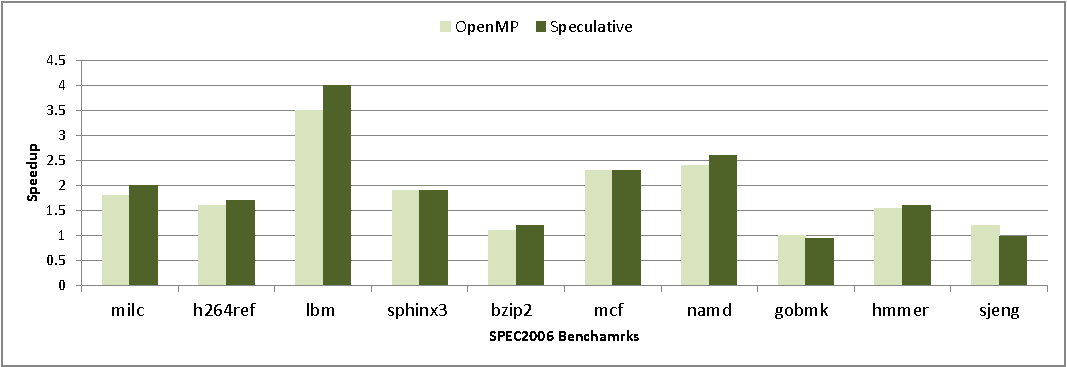
\includegraphics[scale=0.75]{./pdf/openmp_vs_spec}
\caption{Comparison of Speedups gained from OpenMP parallelism done by \textit{Polly} and speculative parallelism for SPEC2006 benchmarks. Speculative parallelization is able to detect more parallelizable loops than OpenMP and gets better speedup. The best improvement is gained for \textit{lbm} as this benchmark has a large loop that can be speculative parallelized but is not parallelized by OpenMP}
\label{fig:openmp_vs_spec}
\end{figure*}

\begin{figure*}[h]
\centering
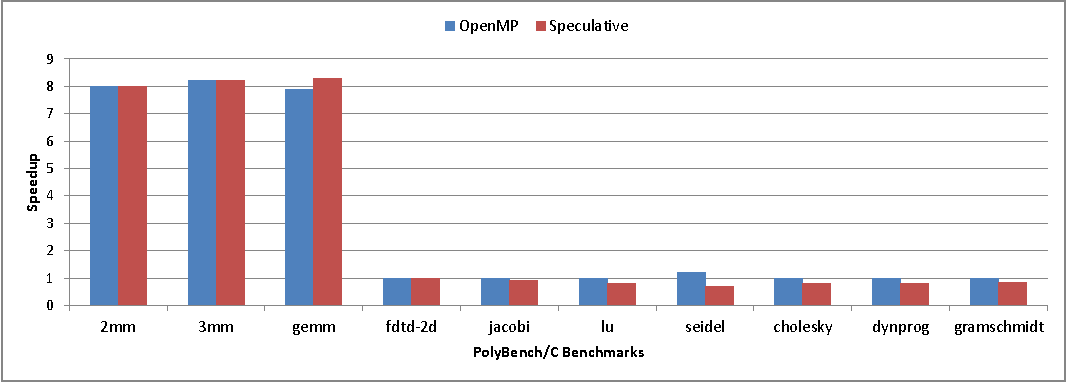
\includegraphics[scale = 0.75]{./pdf/openmp_vs_spec_poly}
\caption{Comparison of Speedups gained from OpenMP parallelism done by \textit{Polly} and speculative parallelism for PolyBench/C benchmarks in a 12-node cluster. The last five benchmarks experiences a slowdown as compared to OpenMP parallelization because the loops parallelized are small and takes very small portion of the total program execution time.  Therefore the speculation overhead negates the performance gained from parallelism.}
\label{fig:openmp_vs_spec_poly}
\end{figure*}

\subsection{Heuristic 2}

\subsubsection{Profiling and Filtering hot loops}

To tackle the slowdowns, the reported \textit{may dependences} are profiled to see whether the dependences occur at run time. Also the loops that does not take significant amount of the program execution time were not speculatively parallelized because they negate the gain of parallelization due to thread creation overhead. \\
The results shown in Figure~\ref{fig:heu2} indicate that the benchmarks that were experiencing slowdown as compared to OpenMP performs equal or better  when heuristic 2 is used. \textit{Gramschmidt} and \textit{sjeng} performs better than OpenMP as the overhead from parallelizing small loops goes away.  This indicates that by extending heuristic 1, equal or better performance can be achieved as compared to OpenMP.

\begin{figure}
\centering
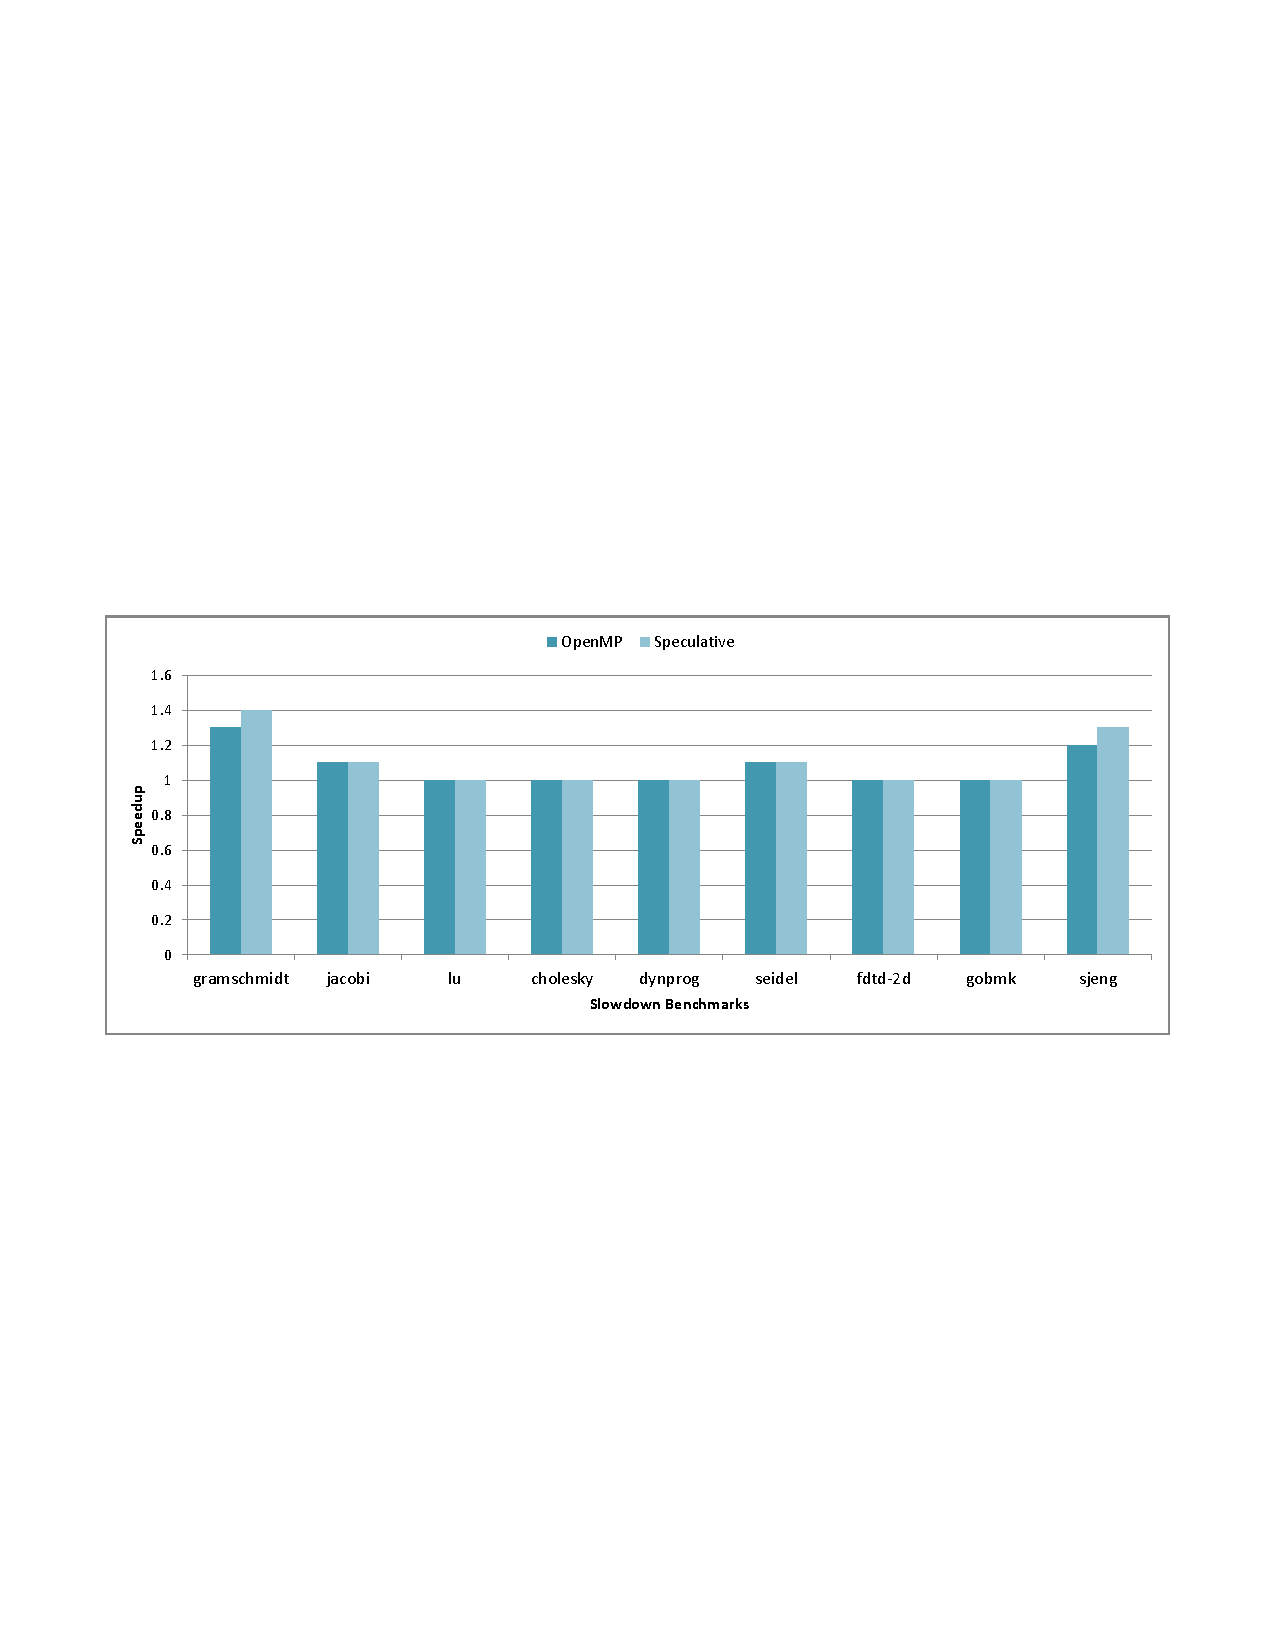
\includegraphics[scale=0.75]{./pdf/heu2.pdf}
\caption{Comparison of Speedups gained from heuristic 2 vs OpenMP for the slowdown benchmarks. Heuristic 2 performs equal or better than OpenMP for \textit{all} cases after profiling dependences and preventing cold loops and loops with a run time dependence. }
\label{fig:heu2}
\end{figure}

In the next chapter, the framework takes the dependence analysis results from the built-in static dependence analyzer of LLVM in stead of the results from \textit{polly} .  The chapter also presents a performance comparison among the automatically SIMDized, automatically OpenMP parallelized code by IBM's \textit{xlc} compiler and speculatively parallelized code by the framework for the SPEC2006 and PolyBench/C benchmarks, using sequential code compiled with the highest optimization level (-O5).

\chapter{Going further:Effect of Higher Optimization Levels of the Compiler and Combining Profiles}
\label{chapter:O5}

\section{Introduction}

The higher optimization levels of the compiler can give many-fold better performance than the sequential code optimized at the lowest level (-O0).  To obtain maximum performance gain from the compiler optimizations, programmers typically use the highest optimization level of a given compiler (e.g. -O5 for IBM's \textit{xlc} compiler, -O3 for \textit{gcc}).\\
To exploit the available parallelism from the programs, different automatic parallelization techniques like automatic OpenMP, automatic SIMDization etc. are used by programmers.  This chapter explores the opportunities of extracting more parallelism from the program using TLS.  The dependence analyzer from LLVM is used to find may dependences inside loops.  A performance comparison of three parallel versions of the code - 1. code generated by the existing automatic OpenMP and 2. SIMD parallelizer of the \textit{xlc} compiler and 3. the speculatively parallel code generated by the framework is presented.  Results show that for some benchmarks (\textit{namd}, \textit{mcf}, \textit{lbm}), TLS gives better performance while for some benchmarks, TLS experiences a performance degradation due to various reasons like - increase in L1 cache misses (\textit{sjeng}, \textit{cholesky}, \textit{dynprog}), instruction path length increase (\textit{jacobi}, \textit{seidel}), misspeculation due to dependences resulting from function calls (\textit{sjeng}, \textit{h264ref}).

\section{Experimental Evaluation}

This section describes the performance evaluation after applying profile-driven TLS to the SPEC2006 and PolyBench/C benchmarks using the LLVM compiler, the BlueGene/Q machine being the platform.  The dependence analysis pass of LLVM is used and the effect of higher optimization level (-O5) of the compiler is observed.  A comparison among three parallel version of the code - SIMDized, automatic OpenMP parallelized and speculatively parallelized is also performed. The benchmarks chosen are widely used in TLS literature.

\section{Comparison with AutoSIMD and AutoOpenMP by the bgxlc\_r compiler}

In this set of experiments, the effect of higher optimization levels of the \textit{bgxlc\_r} compiler is observed.  The optimization level used in both the sequential and parallel version is -O5.  By default -O5 level turns on the automatic vectorization (SIMDization) and the various optimizations of hot loops (e.g. loop unrolling etc.).  \\
Also as LLVM's dependence analysis pass has been improved by the time these experiments are performed, the result from the dependence analysis pass is used for profiling.  The SPEC2006 and PolyBench/C benchmarks are used for experimentation.\\
The baseline for comparison for these set of experiments is the sequential version of the code optimized at the highest level (-O5) with the automatic vectorization and optimization of hot loops turned off.  Comparison is made with three parallel versions of the code.  The automatic SIMDized code, the automatic OpenMP parallelized code and the speculative parallel code generated by the framework.  The following compiler options are used to generate the sequential and the three parallel versions of the code. \\

\begin{itemize}
\item \textbf{Optimized Sequential version:} bgxlc -O5 -qsimd=noauto -qnohot -qstrict 
\item \textbf{Automatic SIMDized version:} bgxlc -O5 -qsimd=auto -qhot -qstrict 
\item \textbf{Automatic OpenMP parallelized version:} bgxlc\_r -O5 -qsimd=auto -qhot -qsmp=auto -qstrict 
\item \textbf{Speculative parallelized version:} bgxlc\_r -O5 -qsimd=auto -qhot -qsmp=auto:speculative -qstrict
\end{itemize}

The \-qstrict compiler option is used to maintain the correct semantics of the program after higher level optimizations because the higher level optimizations may alter the semantics of the program. \\

\begin{figure}[h]
\centering
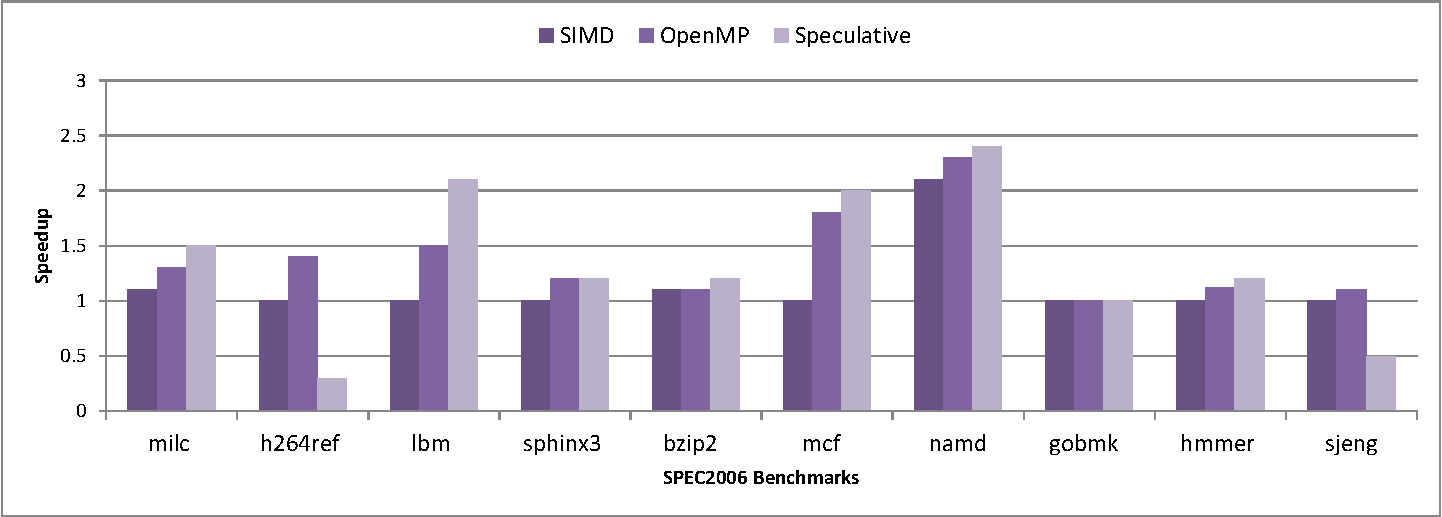
\includegraphics[scale=0.56]{./pdf/spec2006_O5.pdf}
\caption{Comparison of Speedups gained from different parallelization techniques as compared to the sequential version of the code optimized at the highest level for SPEC2006 Benchmarks }
\label{fig:speedup_O5}
\end{figure}

Figure~\ref{fig:speedup_O5} gives the speedup of three parallel versions of the SPEC2006 benchmarks over the sequential version.  As seen in the figure, there are three classes of benchmarks - benchmarks that achieve performance improvement for applying TLS (milc, lbm, bzip2, mcf, namd, hmmer), benchmarks that does not get performance improvement (sphinx3, gobmk) and benchmarks that get a performance degradation after applying TLS (h264ref, sjeng).  \\
Figure~\ref{fig:poly_O5} gives the speedup of the PolyBench/C benchmarks. There are also three classes of benchmarks. lu and gemm gets a performance improvement from TLS while jacobi and dynprog experience slowdown.  Performance does not improve by applying TLS to \textit{2mm}, \textit{3mm}, \textit{fdtd-2d}, \textit{gramschmidt} and \textit{seidel}.\\
One of the reasons for performance improvement are the number of parallelized loops and their coverage (percentage of the loops' execution time with respect to the whole program execution time).  There is limited performance improvement due to TLS for loops that do not have good coverage because of thread creation overhead. bzip2, sjeng are examples of programs that contain speculative loops with poor coverage. \\
Increase in L1 cache misses due to TLS is another reason that limits performance.  In BG/Q, for short-running mode, the L1 cache is flushed before entering any speculative region thus affecting speculative regions with data locality.  Benchmarks such as cholesky and dynoprog suffer from the flush-effect of TLS.\\
The saving of register context before entering in a speculative region, obtaining a speculative ID etc. accounts for the TLS overhead that is reflected in the instruction path length increase.  jacobi and seidel are two benchmarks that experience a huge path length increase thus limiting/degrading their performance.
The rest of the section explains in details the sources
of BG/Q TM overhead.

\begin{figure}[h]
\centering
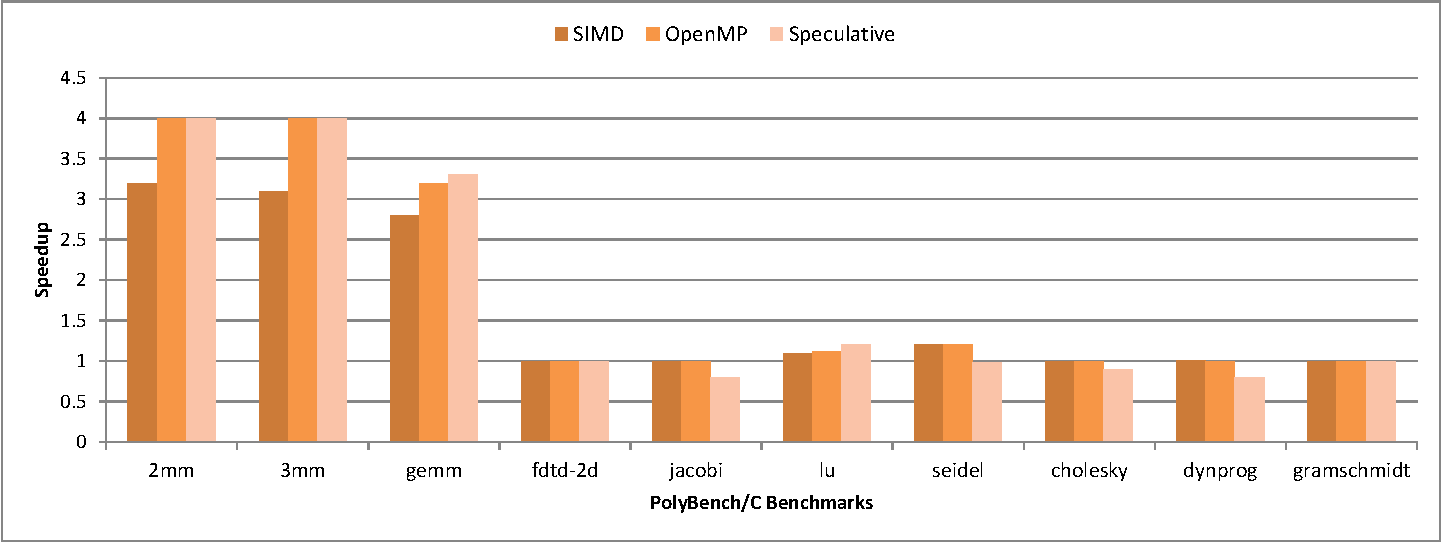
\includegraphics[scale=0.56]{./pdf/poly_O5.pdf}
\caption{Comparison of Speedups gained from different parallelization techniques as compared to the sequential version of the code optimized at the highest level for PolyBench/C Benchmarks}
\label{fig:poly_O5}
\end{figure}


\subsubsection{Investigation of Performance Improvement or Degradation}

The following set of experiments were performed to investigate the reason of performance improvement or degradation due to different parallelization techniques for the SPEC2006 and PolyBench/C benchmarks.  First the number of loops parallelized and their coverage are measured.  Next, the misspeculation overhead of the speculatively parallelized versions are measured in terms of the number of threads squashed due to dependence violation. The L1 cache miss rate of the sequential and the three parallel versions of the code are measured using BG/Q Hardware Performance Monitors (HPM).  Also the instruction path length increase of the parallel versions of the code with respect to the sequential version is calculated.

\subsubsection{Number of loops parallelized and their coverage}

\begin{table}[h]
\centering
\caption{Number of Loops parallelized by different parallel versions of the benchmarks}
\begin{tabular}{|c||c|c|c|c|c|} \hline
Benchmarks & \# Total loops & Speculative & OpenMP & SIMDized & Coverage \\ \hline
lbm & 23 & 5 & 4  &	0 & 98\\ \hline
h264ref & 1870 & 264 & 179 & 3 & 82 \\ \hline
hmmer &	 851	 & 30 & 105 & 17 & 80 \\ \hline
mcf & 52 & 12 & 9 & 0 & 65 \\ \hline
sjeng &	216 & 16	 & 9 & 0 & 32 \\ \hline
sphinx3 & 609 & 2 & 11 & 0 & 91 \\ \hline
bzip2 & 232 & 2 & 4 & 0 & 35 \\ \hline
gobmk & 1265 & 0 & 0 & 0 & - \\ \hline
milc & 421 & 22 & 7 & 2 & 69 \\ \hline
namd & 619 & 25 & 9 & 7 & 92 \\ \hline	
2mm	&20& 7 &7 & 3 & - \\ \hline
3mm	&27& 10&10 & 3 & - \\ \hline	
gemm & 13 & 3 & 4 & 4 & 98 \\ \hline
gramschmidt & 10 & 0 & 3 & 0 & - \\ \hline
jacobi & 9 & 2 & 1 & 0 & 35 \\ \hline
lu & 8 & 5 & 3 & 1 & 45 \\ \hline
seidel & 8 & 2 & 4 & 0 & 40 \\ \hline	
cholesky & 9 & 4 & 0 & 0 & 25 \\ \hline
dynprog & 9 & 3 & 0 & 0 & 26 \\ \hline
fdtd\_2d & 14 & 3 & 0 & 0 & 21 \\ \hline
\hline\end{tabular}
\label{table:coverage_2}
\end{table}

Table~\ref{table:coverage_2} gives the number of parallelized loops by the three different parallelization techniques and their coverage for the SPEC2006 and PolyBench/C benchmarks.  As seen in the table, more loops are parallelized by the automatic OpenMP and speculative parallelization of benchmarks than by \textit{polly}.  The threshold to consider a loop \textit{cold} is still 20\% of the whole program execution time.  More loops are parallelized because \textit{polly} only reports loops that are SCoPs.  For being considered as a SCoP, the loop has to have some specific properties.  These properties prevent \textit{polly} from reporting several loops.  In the later experiments, the dependence analysis results from LLVM are observed and the \textit{may dependent} memory accesses are instrumented for profiling.  Therefore, the cardinality of the set of loops profiled increases that results in an increase in the number of loops reported to be beneficial based on the speculative candidate loop selection criteria.\\
The number of loops parallelized by the auto-OpenMP parallelization in the \textit{bgxlc\_r} compiler is also greater than the number of loops parallelized by \textit{polly} using the polyhedral dependence analysis because \textit{polly} only considers SCoPs where \textit{bgxlc\_r} takes all loops (non SCoPs as well) while performing the dependence analysis.\\
Apart from including non-SCoPs, there is one more relaxation for finding the speculation candidates.  Loops with function calls inside their body are considered to be speculatively parallel if the all the memory accesses (apart from the function call) inside the loop body are independent.  Even if the function call introduces dependency inside the loop, that dependency is not checked.  The reason for this relaxation is - it is difficult to perform an inter-procedural dependence analysis with the help of profiling.  A more conservative compiler does not consider a loop as a candidate for speculation if there is a function call inside the loop body and the function is not side-effect free. \\
The interesting benchmark in table~\ref{table:coverage_2} is \textit{h264ref} because it has the highest number of speculatively parallelized loops with good coverage than any other benchmark but still it experiences a slowdown due to speculative execution, as seen in figure~\ref{fig:speedup_O5}.  The reason for this slowdown in investigated further. \\ \textit{milc} has a large number of speculative loops that do not have a high coverage and the performance improvement from TLS execution is limited by this fact.  The coverage of the speculative loops in \textit{sjeng} is low and the poor coverage introduces TLS thread creation overhead that in turn results in a slowdown.  The number of loops speculatively parallelized for \textit{lbm} is small but they take a significant portion of the whole program execution time (98\%).  These hot loops of \textit{lbm} are good speculation candidates and are examples of cases where TLS can be beneficial. \\ \textit{namd} have decent number of speculated loops with a good coverage which contributes to the speed up from TLS.  \textit{bzip2} has a small number of loops that does not have good coverage, therefore asking for investigation of other reasons for the perfromance improvement of this benchmark. \textit{gobmk} does not have any parallelizable loops for either SIMDization, automatic OpenMP and TLS parallelization. Therefore the benchmark takes the same time as the optimized sequential version, as seen in figure~\ref{fig:speedup_O5}. \\
For PolyBench/C benchmarks, \textit{2mm} and \textit{3mm}, no new speculation candidate loops are discovered than automatic OpenMP parallelization because these benchmarks are matrix multiplication benchmarks that contain large parallelizable loops.  These loops are parallelized by automatic OpenMP parallelizer. For \textit{gemm}, the speculatively parallel loops have good coverage that accounts for the performance improvement from TLS.  For \textit{cholesky}, \textit{dynprog} and \textit{fdtd-2d} the loops paralleized have poor coverage that results in a performance degradation. \textit{gramschmidt} does not have any speculative loops discovered because the \textit{cold} loops (less than 20\% coverage) that are parallelized by the \textit{polly} framework are filtered out.

\subsubsection{Misspeculation Overhead}
\label{sec:mispeculation}
Squashing of threads with dependence and re-execution the parallel section sequentially imposes overhead that results in performance degradation of programs.  For speculatively parallelizing loops with function calls, new dependences may be introduced that lead to dependence violation and thread squashing.  The measurement of misspeculation overhead identifies loops inside benchmarks where function calls introduce actual dependences during run-time.\\
To measure the misspeculation overhead, the percentage of successfully committed threads are computed.  The \textit{se\_print\_stats} function from the \textit{speculation\.h} header file in BG/Q is used to collect various statistics for a speculative region including the number of successfully committed/non-committed threads.  The \textit{se\_print\_stats} function is inserted before and after each speculative loop.  An environment variable can be set to print the statistics either after each speculative regions or from all the speculative regions at the end of the program.  The percentage of speculative threads committed is computed using the following equation:

\begin{equation}
 \frac{speculative }{\left ( speculative + non\_speculative \right )}\ast 100
\end{equation}

\begin{table}[h]
\centering
\caption{The percentage of Speculative Threads successfully committed (not rolled back) for SPEC2006 and PolyBench/C Benchmarks.  It gives the amount of wastage computation. Data is omitted for the benchmarks that has no discovered speculative loop }
\begin{tabular}{|c||c|} \hline
Benchmark &Percentage of Speculative Committed\\ \hline 
lbm &  94\\ \hline
h264ref & 12  \\ \hline
hmmer &	79	  \\ \hline
mcf & 88 \\ \hline
sjeng &	8 \\ \hline
sphinx3 & 29  \\ \hline
bzip2 & 78  \\ \hline
gobmk & -  \\ \hline
milc & 79  \\ \hline
namd & 80  \\ \hline
2mm	& - \\ \hline
3mm	& - \\ \hline
gemm	 & 89 \\ \hline
gramschmidt	& - \\ \hline
jacobi & 78 \\ \hline
lu	& 89 \\ \hline
seidel&	70 \\ \hline
cholesky & 79 \\ \hline
dynprog & 82 \\ \hline
fdtd\_2d & 68 \\ \hline
\hline\end{tabular}
\label{table:spec_committed}
\end{table}

The percentage of successfully committed threads gives an idea about the amount of wasted computation for the speculative loops.  Ideally a benchmark that can be benefited from TLS should have high percentage of successful completion of speculative threads. Table~\ref{table:spec_committed} gives the percentage of speculative threads committed for the SPEC2006 and PolyBench/C benchmarks.  The best TLS performance in terms of successful thread completion is given by \textit{lbm}.  For \textit{sjeng} and \textit{h264ref} the percentage of speculative threads committed is pretty less giving an indication of a huge amount of wasted computation that result in their slowdown.  Closer investigation of these benchmarks reveal that most of the loops speculatively parallelized contains function calls that result in a dependence and thus cause a roll back.  Though \textit{h264ref} has the most number of loops speculatively parallelized, the presence of dependence resulted from the function calls inside the loops results in the slowdown. The following can be used to overcome the misspeculation overhead due to function calls:
\begin{itemize}
\item The compiler can be conservative and may not allow loops with function calls inside them to be executed in parallel regardless of whether the function call changes the dependence behaviour of the loop.  In this heuristic, we might still miss some opportunities where the function call is harmless.
\item A more sophisticated inter-procedural dependence analysis technique can be used that is able to tell if the function call introduces new dependences in of the loop.
\end{itemize}
\textit{mcf}, \textit{hmmer}, \textit{milc}, \textit{namd} and \textit{bzip2} do not have a high percentage of successful speculative execution because these benchmarks have some loops with function calls introducing dependence.  The misspeculation percentage explains the small performance improvement over OpenMP parallelization for these benchmarks as compared to \textit{lbm}.\\
Among the PolyBench/C benchmarks, \textit{gemm} and \textit{lu} has high percentage of speculative thread completion that accounts for their speedup.  For the four benchmarks - \textit{jacobi}, \textit{seidel}, \textit{cholesky}, \textit{dynprog} there is high percentage of thread completion but still these benchmarks result in slowdown.  The reason of performance degradation for these four benchmarks is investigated further.

\subsubsection{L1 Cache Miss Rate}

The TLS runtime works in close collaboration with the Transactional Memory (TM) runtime of BG/Q.  One of the most dominant BG/Q TLS runtime overhead is caused by the loss of L1 cache support due to the L1 flush and bypass needed for the bookkeeping of speculative
state in L2. Though the L2 and L1P buffer load latencies are 13x and 5x higher than the L1 load latency, the L1 miss rate for the sequential ans different parallel versions of the code gives an idea about the performance gain or loss for the benchmarks.\\
The Hardware Performance Monitor (HPM) library of BlueGene/Q is used to collect these statistics. Table~\ref{table:cache} gives the L1 cache misses for the sequential version and the three parallel versions of the SPEC2006 and PolyBench/C benchmarks.\\

\begin{table}[h]
\centering
\caption{\#L1 Cache Hit Rate for SPEC2006 and PolyBench/C benchmarks}
\begin{tabular}{|c||c|c|c|c|} \hline
Benchmark &Sequential & SIMD & AutoOMP & Speculative\\ \hline 
lbm & 95 & 94 & 94 & 93\\ \hline
h264ref & 96 & 95 & 95 & 94 \\ \hline
hmmer &	98 & 97 & 97 & 95  \\ \hline
mcf & 92 & 92 & 95 & 95 \\ \hline
sjeng &	96 & 96 & 95 & 90 \\ \hline
sphinx3 & 96 & 96 & 95 & 95  \\ \hline
bzip2 & 95 & 95 & 95 & 97  \\ \hline
gobmk & 97 & 97 & 97 & 97  \\ \hline
milc & 95 & 97 & 97 & 98  \\ \hline
namd & 96 & 98 & 97 & 98  \\ \hline
2mm	& 98 & 98 & 99 & 99 \\ \hline
3mm	& 98 & 98 & 99 & 99 \\ \hline
gemm	 & 98 & 96 & 98 & 98\\ \hline
gramschmidt	& 97 & 97 & 97 & - \\ \hline
jacobi & 97& 97 & 97 & 97 \\ \hline
lu	& 96 & 96 & 95 & 96 \\ \hline
seidel&	98 & 97 & 98 & 98 \\ \hline
cholesky & 98 & 98 & 96 & 88\\ \hline
dynprog & 97 & 96 & 97 & 90\\ \hline
fdtd\_2d & 98 & 98 & 98 & 98 \\ \hline
\hline\end{tabular}
\label{table:cache}
\end{table}

For \textit{lbm}, the three parallel versions of the code results in more L1 cache misses thus limiting the performance improvement.  But for \textit{mcf}, both automatic OpenMP and speculative versions result in higher L1 hits which contributes to the performance improvement.  The speculative execution of \textit{sjeng} also results in a high L1 miss rate.  This is the effect of flushing the L1 cache before entering TLS region in the long-running mode.  Apart from the function calls inside TLS regions which introduce data dependences (Table ~\ref{table:spec_committed}, the high L1 miss rate affects the performance for \textit{sjeng}.\\
Similar effect can be seen for the two PolyBench/C benchmarks - \textit{cholesky} and \textit{dynprog}.  Though these two benchmarks have high percentage of successful completion of speculative threads as seen in table~\ref{table:spec_committed}, the speculative execution of the selected loops affects the cache performance due to locality of data between threads.  The cost of bringing the data again after flushing the cache accounts for the slowdown in these benchmarks. \\
For \textit{jacobi} and \textit{seidel} benchmarks, though the speculative execution of the loops result in better cache utilization, the benchmarks experiences a slowdown.  The reason for this slowdown is investigated further.  The two benchmarks \textit{fdtd-2d} and \textit{gobmk} does not show any change in cache utilization for the three parallelization techniques, because the three parallelization techniques, due to discovery of no parallelizable loops, do not perform any code transformation than the optimized sequential version.

\subsubsection{Instruction Path length increase}

Automatic OpenMP and speculative parallelization inserts call to OpenMP and TLS runtime functions respectively before and after speculative loops.  Code also needs to be inserted for saving the consistent system state so that the system can be rolled back to a previous state in case of a dependence violation.  Code growth may also occur for SIMD parallelized version of the code due to insertion of new instructions and also for applying different loop optimizations (e.g loop unrolling) performed with the -qhot option.  The effect of the three parallelization techniques on code growth is observed and the results are given in table~\ref{table:instruction_path}.\\

\begin{table}[h]
\centering
\caption{Instruction Path Length Increase With Respect to Sequential Version for SPEC2006 and PolyBench/C benchmarks}
\begin{tabular}{|c||c|c|c|} \hline
Benchmark & SIMD & AutoOMP & Speculative\\ \hline 
lbm & .03 \% & .25 \% & 26 \%\\ \hline
h264ref & .6 \% & 15 \% & 56 \% \\ \hline
hmmer  & 10 \% & 35 \% & 37 \%  \\ \hline
mcf  & 0 \% & 12 \% & 23 \% \\ \hline
sjeng  & 0 \% & 0 \% & 45 \%  \\ \hline
sphinx3  & 0 \% & 18 \% & 19 \%  \\ \hline
bzip2 & 0 \% & 2 \% & 3 \%  \\ \hline
gobmk  & 0 \% & 0 \% & 0 \%  \\ \hline
milc  & 0.9 \% & 12 \% & 23 \%  \\ \hline
namd & 1 \% & 12 \% & 25 \%  \\ \hline
2mm	& 13 \% & 45 \% & 45 \% \\ \hline
3mm	 & 13 \% & 46 \% & 46 \% \\ \hline
gemm	  & 11\% & 45 & 45 \% \\ \hline
gramschmidt	 & 0 \% & 46 \% & 46\% \\ \hline
jacobi & 0 \% & 95 & 112 \%  \\ \hline
lu	 & 1 \% & 12 \% & 13 \% \\ \hline
seidel&	 0.02 \% & 98 \% & 123 \% \\ \hline
cholesky  & 0 \% & 0 \% & 39 \%\\ \hline
dynprog& 0 \% & 0 \% & 75 \%\\ \hline
fdtd\_2d  & 0 \% & 0 \% & 79 \% \\ \hline
\hline\end{tabular}
\label{table:instruction_path}
\end{table}

As seen in the table~\ref{table:instruction_path}, the code growth for PolyBench/C benchmarks is larger than the SPEC2006 benchmarks.  The code growth is due to loops constituting major portion of the PolyBench/C benchmarks. Applying optimizations to the loops effects the code size the most.  For SPEC2006 benchmarks the code growth is relatively smaller than PolyBench/C benchmarks, the highest being for the speculative parallelization of the \textit{h264ref} benchmark because a large number of loops are speculatively parallelized for this benchmark. \\
\textit{jacobi} and \textit{seidel} from the PolyBench/C benchmarks experience a massive code growth that explains their slowdown.  The code growth is due to two different reasons - 1. The loops parallelized constitute the maximum code portion of the benchmark. 2. The memory footprint of the loops speculatively parallelized are large and therefore, saving register context for speculative execution of the loops adds a significantly large number of instructions to these two benchmarks.

\section{Filtering Loops with Function Calls that have Side Effects }

Section~\ref{sec:mispeculation} shows that for some benchmarks (\textit{h264ref}, \textit{sjeng}), allowing speculative execution of loops with function calls introduces huge misspeculation overhead that results in slowdown.  The function calls inside the loop bodies introduce dependences across iterations of the loop.  Static analysis of the compiler was not able to detect these dependences.  Inter-procedural dependence analysis with the help of profiling is hard to do, therefore, these dependences are also not detected through runtime dependence profiling.  There can be two solutions to overcome the overhead: 
\begin{itemize}
\item Perform a more sophisticated compile-time inter-procedural dependence analysis to discover these dependences.
\item Use a conservative heurisitic to not allow the speculative execution of loops that has non-side-effect-free function calls inside their body.
\end{itemize}
In this section, the impact of using the second option on the performance of the loops in the SPEC2006 and PolyBench/C benchmarks is explored. 
\begin{figure}[h]
\centering
\includegraphics[scale=0.56]{./pdf/spec_modified.pdf}
\caption{Performance does improves for the modified heuristic for SPEC2006 benchmarks because the loops that were having dependence due to to function calls are not executed speculatively in parallel.  There is not performance degradation indicating that independent loops that have function calls do not impact the performance of the SPEC2006 benchmarks.}
\label{fig:spec_modified}
\end{figure}
As seen in figure~\ref{fig:spec_modified}, not allowing loops with non-side-effect-free function calls have a huge performance impact on the \textit{h264ref} and \textit{sjeng} benchmarks.  The percentage of successfully committed threads jumps up from 12\% to 96\% for \textit{h264ref} and from 8\% to 97\% for \textit{sjeng}.  Using this heuristic also improves the performance for \textit{hmmer} because hmmer also contains some loops where dependence is introduced due to function calls.  Performance does not degrade for any of these benchmarks indicating that execution of loops with non-side-effect-free function calls that do not introduce dependence are not significant for these benchmarks. \\
As seen in figure~\ref{fig:poly_modified}, the performance of the PolyBench/C benchmarks does not change for using the heuristic.  Mostly PolyBench/C benchmarks are kernel benchmarks and the loops inside them do not contain function calls.



\begin{figure}[h]
\centering
\includegraphics[scale=0.56]{./pdf/polly_modified.pdf}
\caption{Performance does not change for the modified heuristic for PolyBench/C benchmarks because the loops inside them are small kernel loops that do not contain function calls}
\label{fig:poly_modified}
\end{figure}

\chapter{Conclusion}
\label{chapter:conclusion}

TODO
\chapter{Related Work}
\label{chapter:related work}

This chapter summarizes the previous research on Thread level speculation.  Related work on the use of data dependence profiling for TLS is also summarized.  Section 1 summarizes the previous work on TLS while Section 2 gives related work on the use of data dependence profiling in TLS.

\section{Thread Level Speculation}

One of the earlier works on TLS is based on Address Resolution Buffers (ARB) by Franklin \textit{et al}~\cite{ARB}.  They propose a hardware mechanism, ARB for performing dynamic reordering of memory references.  ARB has support for the following features - 1) dynamic disambiguation of memory references 2) multiple memory references per cycle, 3) out-of-order execution of memory references, 4) unresolved loads and stores, 5) speculative loads and stores, and 6) memory renaming. ARB is a shared table that is used to track speculative loads and stores.  The scheme allows speculative loads and speculative stores by keeping the uncommitted store values in the hardware structure and forwarding them to subsequent loads that require the value.\\
Following the work by Franklin \textit{et al.}, multiple proposals have been made to move speculative data into each core's private cache or write buffer, and use the cache coherence protocols for memory disambiguation.   In contrast to ARB that uses a centralized buffer to support speculative versions, the work of Vijaykumar \textit{et al.}, called the \textit{Speculative Versioning Cache (SVC)}, uses distributed caches to eliminate the latency and bandwidth problems of the ARB~\cite{Gopal}. The SVC approach is based on unification of cache coherence and speculative versioning by using an organization similar to snooping bus-based coherent caches. Memory references that gets a hit in the private cache do not use the bus as in an SMPs. The committed tasks do not write back the speculative versions all at one time. Instead, versions are marked, together, as committed at commit time, without performing any data movement. Each cache line is individually handled when it is accessed the next time.\\
Lance Hammond \textit{et al.} describes the implementation of speculative execution in a chip multi-processor (CMP), called Hydra~\cite{Hydra}. Their approach a hardware+software hybrid mechanism (a number of software speculation control handlers and modifications to the shared secondary cache memory system of the CMP) to achieve TLS. Their results show that TLS is profitable for applications with substantial amount of medium-grained loops.  When the granularity of parallelism is too small or the available \textit{inherent} parallelism in the application is low, the overhead of the software speculation handlers overwhelms the potential performance benefits from TLS.\\
Steffan \textit{et al.} proposes and evaluates a TLS system that scales to any machine size.  Their strategy is a straightforward extension of writeback invalidation-based cache coherence~\cite{steffanISCA00}. The scheme has 1. a notion of whether a cache line has been speculatively loaded and/or speculatively modified; 2. a guarantee that a speculative cache line will not be propagated to regular memory, and that speculation will fail if a speculative cache line is replaced.  They add three new speculative coherence messages and speculative cache states in the cache coherence protocol.  They show that using their model, applications scale from single-chip multiprocessors or simultaneously multi-threaded processors up to large-scale machines which might use single-chip multiprocessors.\\
Luis Ceze \textit{et al.} describes an approach to disambiguate memory references so that the dependences in the code can be checked during program execution and threads can be committed or rolled back accordingly~\cite{bulk}.  They hash-encode a thread's access information in a \textit{signature}, and then add operations that efficiently process sets of addresses from the signature.  They employ a \textit{Bloom-filter-based} compact representation of a thread's access information.  They call their mechanism \textit{Bulk} operation as they operate on a set of addresses.  They show that, despite its simplicity, \textit{Bulk} has competitive performance with more complex schemes.\\
Steffan\textit{ et al.} shows that the performance of a TLS system is dependent on the way threads communicate values among them~\cite{value_communication}.  They apply three different actions - value prediction, dynamic synchronization, and hardware instruction prioritization to improve value communication among threads. Their technique first explores how \textit{silent stores} (value of the memory location before the store is the same as the value of the location after the store) can be exploited within TLS. The TLS system avoids data dependence violations and makes dependent store-load pair independent if the store is silent.  In this way the TLS system reduces the coherence traffic as well as future update traffic. The silent store approach yields similar performance to value predictors but requires less complex design.  They also use some compiler heuristics to select loops for TLS (based on the execution time, number of iterations of the loop etc.) and apply compiler optimization (e.g loop unrolling, reducing critical forwarding path of values between loop iterations etc.) that significantly improves TLS performance.\\

\subsubsection{Loop Selection for Speculative Execution}

Because loops are normally targeted for TLS, different heuristics are proposed to select candidate loops for speculative execution.\\
Colohan \textit{et al.} empirically studies the impact of thread size on the performance of loops~\cite{colohan1}. They employ different techniques to unroll loops in order to determine the best thread size per loop. They also propose a run-time system to measure the performance and select each loop dynamically. Due to the run-time overhead, the system can only select loops locally without considering loop nesting.\\
Oplinger \textit{et al.} proposes and evaluates a static loop selection algorithm using simulation~\cite{olukotun}. In their algorithm, they select the best loops in each level of dynamic loop nest as possible candidates to be parallelized and then compute the frequency with which each loop is selected as best loop. Finally, they select the parallelized loops based on the computed frequencies. The concept of dynamic loop nest is similar to the loop tree proposed in our study. However, this technique is only used to guide the heuristic in context-insensitive loop selection. Their performance estimation is obtained directly from simulation, and does not consider the effect of compiler optimization.\\
Chen \textit{et al.} proposes a dynamic loop selection framework for Java program~\cite{chen1}. They use hardware to extract useful information, such as dependence timing, and speculative state requirements and then estimate the speedup for a loop. Their technique is similar to the runtime system proposed by Colohan \textit{et al.} and can only select loops within a simple loop nested program. Considering the global loop nesting relations and selecting the loops globally introduces significant overhead for the run-time system.\\
Marcuello \textit{et al.} proposes a thread spawning scheme that supports spawning threads from any point in the program~\cite{marcuello}. They use profile information to identify appropriate thread spawning points with more emphasis on thread predictability.\\
Wang \textit{et al.} proposes different techniques to select loops for TLS~\cite{loopselection}.  They use a construct called \textit{loop-graph} that describes the different nesting relations among loops.  Only one loop from a loop nest is parallelized based on some heuristics.  They use run-time profile information to measure the performance improvement of parallelizing a loop.  They also apply graph-pruning to reduce the "selection problem" size (which is otherwise NP complete).  Most importantly, they show that the dynamic behaviour of a loop is sensitive to its calling context (for some invocation, the loop may gain performance improvement and for some, it may not).  They attach the calling context information in the loop graph.

\section{Data Dependence Profiling for TLS}

The necessity of data dependence profiling to find TLS candidate loops that cannot be discovered by static dependence analysis is explored.  This section describes the previous work on data dependence profiling and the use of it in the case of TLS.\\
Ju \textit{et al.} proposed a unified framework to exploit both data and control speculation targeting specifically for memory latency hiding~\cite{ju_spec}. The speculation is exploited by hoisting load instructions across potentially aliasing store instructions or conditional branches.  The framework also contains recovery model which relies on compiler-generated explicit recovery blocks.  Their framework shows modest performance improvement in SPECInt95 benchmarks by shortening critical paths despite some side effects, such as recovery code penalty during misspeculation and higher register pressures.\\
Chen \textit{et al.} propose a data dependence profiler targeted at speculative optimizations~\cite{chen_spec}. They perform speculative Partial Redundancy Elimination (PRE) and code scheduling, using a naive profiler and speculative support provided through the ALAT (Advanced Load Address Table) in the Itanium processors. Their non-sampling profiler has a slowdown of up to 100x, and they propose sampling techniques to overcome this problem. They use a shadow space with a simple hashing scheme to facilitate fast address comparison for detecting data dependences.\\
Lin \textit{et al.} propose a compiler framework for speculative analysis and optimizations~\cite{lin_spec}.  The framework is based on a speculative SSA (Static Single Assignment) form to incorporate speculative information for both data and control speculation.  Speculative SSA integrates the alias information directly into the intermediate representation using explicit \textit{may modify operator} and \textit{may reference operator}. Their speculative analysis is assisted by both \textit{alias profiles} and heuristic rules.\\
The Multiscalar compiler selects tasks by walking the Control Flow Graph (CFG) and accu-
mulating basic blocks into tasks using a variety of heuristics~\cite{multiscalar}. The task selection methodology for the Multiscalar compiler is revisited by Johnson \textit{et al}~\cite{mincut}.  Instead of using a heuristic to collect basic blocks into tasks, the CFG is annotated with weights and broken into tasks using a min-cut algorithm. These compilers assume special hardware for dispatching threads; they do not specify when a thread should be launched.\\
In SPSM, loop iterations are selected by the compiler as speculative threads~\cite{SPSM}. They use a special instruction \textit{fork} that allows the compiler to specify when tasks begin executing. In addition, SPSM recognizes the potential benefits from prefetching but proposes no techniques to exploit it. \\
Bhowmik and Franklin build a framework for speculative multithreading on the SUIF-MachSUIF platform~\cite{bhowmik}. Within this framework, they consider dependence-based task selection algorithms. Like Multiscalar, they focus on compiling the whole program for speculation, but allow the compiler to specify a spawn
location as in SPSM.\\
Du \textit{et al.} propose a cost-driven compilation framework to perform speculative parallelization~\cite{du_spec}. The compiler uses dependence profile for task selection and for partitioning speculative loops into serial and parallel portions. The profiler tracks both intra- and loop-carried- true dependences for speculative loops. Loop-carried-dependences are used to guide the parition of loop bodies into a serial and a parallel portion. Since dependences originated from the serial portion do not trigger roll-back in the parallel portion, the key part of their framework is to move source computation of frequent dependences (called violating candidate) to the serial portion through instruction reordering. A cost model is used to select the optimal loop partition, which is based on the size of serial portion and the misspeculation cost of the parallel portion. The latter is computed by combining re-execution cost of individual nodes weighted by probabilities of carried-dependences (for violating candidates) and intra-iteration dependences (for others).  They achieve a 8\% speedup for the SPECInt2000 benchmarks.\\
Quinones \textit{et al.} evaluated the Mitosis compiler for exploiting speculative thread-level parallelism~\cite{mitosis}.  Mitosis compiler uses both dependence and edge-profiles for 1. generating speculative precomputation slices (p-slice) and 2. selecting spawning pairs. P-slice predicts live-in values for speculative tasks and contributes to the serial portion of the speculative execution. To minimize p-slice overhead while maximizing the accuracy, the compiler uses dependence- and edge-profiles to prune instructions in p-slices. To select spawning pairs, another profile analyzes the sequential execution trace to model the speculative execution time of each candidate spawning pair without considering inter-task memory conflicts. Instead, in this execution model, task squashes is mostly determined by mispredication probability of p-slices. They get a 2.2x speedup for the OLDEN benchmarks on their simulator.\\
Wu \textit{et al.} propose a cost model for compiler-driven task selection for TLS~\cite{dprof}.  The model employs profile-based analysis of may-dependences to estimate the probability of successful speculation.  Their profiling tool, \textit{DProf}, is able to  measure dependence probability and independence window of loops. They provide two techniques - dependence windows (the number of iterations that can be executed in parallel without affecting the output) and dependence clustering (regions of the loop's iteration space with large independence windows that makes that portion profitable to execute in parallel).  One improtant finding is that there is little variability in independence window width in the hot loops for the SPEC2000 benchmarks. Loops are either parallel or serial with an independence window width of 1.\\
Kim \textit{et al.} propose a scalable approach to data-dependence profiling that addresses both runtime and memory overhead in a single framework~\cite{sd3}.  Their technique, called \textit{SD3}, reduces the runtime overhead by parallelizing the dependence profiling step itself. To reduce the memory overhead, they compress memory accesses that exhibit stride patterns and compute data dependences directly in a compressed format. For stride detection, they use a \textit{finite state machine} (FSM).SD3 reduces the runtime overhead by a factor of  9.7× on  32 cores and reduces memory consumption by 20x with a 16x speedup in profiling time.  They also show that the dependence behaviour for different inputs \textit{does not} change for OmpSCR benchmarks and changes very less (correlation 0.98 among the dependence pairs discovered in the loops) for SPEC2006 benchmarks.  This finding is important and supports the findings of my research.\\
POSH is a TLS compiler built on top of gcc~\cite{posh}. POSH performs a partitioning of the code into TLS tasks and considers both subroutines and loops. POSH also uses a simple profiling pass to discard ineffective tasks.  While choosing tasks beneficial for speculation, POSH considers the task size and the squash frequency which is obtained by simulation of the parallel execution.  L2 cache misses are also considered by the profiler to perform prefetching analysis.\\
Vanka \textit{et al.} approaches data dependence profiling from a set-based approach~\cite{vanka}.  Rather than tracking pair-wise dependences, they identify important dependence relationships at compile time, group said relationships into sets, and then construct and operate directly on the sets at runtime.  They use \textit{Signatures}, an efficient set representation based on Bloom filters, to to trade-off performance and accuracy.\\
None of these approaches provide a solution for loops which has varied dependence behaviour for different executions or gives a solution to the problem of combining multiple data dependnece profiles obtained using different inputs to the program.


%\include{Chapters/introduction}



%
%\include{Chapters/related-work}
%
%\include{Chapters/contrib1}
%
%\include{Chapters/contrib2}
%
%\include{Chapters/experiments}
%
%\include{Chapters/conclusions}

\clearpage\addcontentsline{toc}{chapter}{Bibliography}
     %add the above line to get "Bibliography" in the table of contents.
%
\singlespacing % optional;  Bibliography is better in single spacing
               %            but you may choose different
               %            Don't use \singlespacing if your thesis
               %            is already in single spacing
%
\bibliographystyle{plain} % Or which ever you wish. Plain is good
                          % for long bibs.
\bibliography{arnamoy}

\doublespacing

\appendix  %  If you have any appendices
            % Use standard Latex sectioning commands
            % like \chapter etc.

%\include{Chapters/app1}

\end{document}
